\documentclass[letterpaper,twocolumn]{article}

\usepackage{bigdelim}
\usepackage[top=1in,bottom=1in,left=0.75in,right=0.75in]{geometry}
\usepackage{graphicx}
\usepackage{makecell}
\usepackage{multirow}
\usepackage{newtxtext}
\usepackage{newtxmath}
\usepackage{pifont} % For checkmarks in tab:nat-matching.
\usepackage[hyphens]{url}
\usepackage[table]{xcolor}

\usepackage[textsize=footnotesize]{todonotes}\setlength{\marginparwidth}{1.5cm}

% Better look for citations that include a section reference like \cite[\S 3]{foobar}.
\usepackage{cite}
\renewcommand{\citemid}{~}

% Load hyperref after other packages.
\usepackage[pdfa,hidelinks,pdfcreator={},pdfproducer={}]{hyperref}
\urlstyle{same}
\def\sectionautorefname{Section}
\def\subsectionautorefname{Section}

% Disable metadata for reproducible PDF.
% https://tex.stackexchange.com/a/313605
\usepackage{ifpdf}
\ifpdf
\pdfinfoomitdate=1
\pdftrailerid{}
\pdfsuppressptexinfo=-1
\fi

\hyphenation{Web-RTC}
\hyphenation{Web-Exten-sion}
\hyphenation{Java-Script}
\hyphenation{uProxy}
\hyphenation{off-line}
\hyphenation{mac-OS}

% Highlight the first usage or definition of a technical term.
% Like the firstterm element in DocBook: https://tdg.docbook.org/tdg/5.2/firstterm.html.
\newcommand{\firstterm}[1]{\textit{#1}}

\begin{document}

\date{}

\title{Snowflake, a censorship circumvention system \\using temporary WebRTC proxies}

\author{}

\maketitle

\begin{abstract}
Snowflake is a system for circumventing Internet censorship.
It~derives its blocking resistance from
the use of numerous, ultra-light, temporary proxies (``snowflakes''),
which accept traffic from censored clients using peer-to-peer WebRTC protocols
and forward it to a centralized bridge,
which does the real work of directing traffic to its destination.
The temporary proxies are lightweight enough to be implemented in JavaScript,
in a web page or browser extension,
making them vastly cheaper to set up than
a traditional proxy or VPN server.
The proxies are not assumed to have stable network addresses
or be online all the time,
and even the blocking of the currently in-use proxy
is not fatal to a circumvention session,
as the system permits clients to switch proxies on the fly.

% Need anything about broker, centralization here?

Snowflake has been deployed with success
in Tor Browser and Orbot for several years.
It has been significant for circumvention
during high-profile network disruptions,
including in Russia in~2021 and Iran in~2022.
In this paper, we explain the composition of Snowflake's many parts,
give a history of deployment and attempts to block~it,
and reflect on implications for circumvention generally.
\end{abstract}

% General references:
%   https://keroserene.net/snowflake/technical/#history
%   https://www.bamsoftware.com/papers/thesis/#chap:snowflake

\section{Introduction}
\label{sec:intro}

Censorship circumvention systems,
which seek to enable network communication
despite interference by a censor,
may be characterized on multiple axes.
Some systems imitate a common network protocol;
others transform their traffic randomly, in order
not to look like any protocol in particular.
Some distribute connections over numerous proxy servers;
others concentrate on just one proxy
that is, for one reason or another, difficult for a censor to block.
What all circumvention systems have in common
is that they strive to increase the \emph{cost}
to the censor of blocking them---whether that cost be in
research and development, human resources, and hardware;
or in the inevitable overblocking that results
when a censor tries to selectively block
some connections but not others.
Snowflake, the subject of this paper,
is a circumvention system that
uses thousands of temporary proxies
and makes switching between them easy and fast.
On~the spectrum of imitation to randomization,
Snowflake falls on the side of imitation;
on the scale from diffuse to concentrated, it is diffuse.
What most sets Snowflake apart is that
it pushes the idea of distributed, disposable
proxies to an extreme:
its~proxies can run in a web browser
and censored clients communicate with them using WebRTC.

WebRTC is a suite of protocols
intended for real-time communication applications
in web browsers~\cite{rfc8825}.
Video and voice chat are typical examples
of WebRTC applications.
Snowflake exchanges WebRTC data formats
in the course of establishing a connection,
and uses WebRTC protocols for traversal of NAT (network address translation)
and communication between clients and proxies.
Crucially for Snowflake, WebRTC APIs
are available to JavaScript code in web browsers,
meaning it is possible to implement a proxy
in a web page or browser extension.
WebRTC is also usable outside a browser,
which is how we implement the Snowflake client program
and alternative, command line--based proxies.

As~is usual in circumvention research,
we assume a threat model in which
\firstterm{clients} reside in a network
controlled by a \firstterm{censor}.
The censor has the power to inspect and interfere with
traffic that crosses the border of its network;
typical real-world censor behaviors include
inspecting IP addresses and hostnames,
checking packet contents for keywords,
blocking IP addresses, and injecting false DNS responses
or TCP RST packets.
The client wants to communicate with some
\firstterm{destination} outside the censor's network,
possibly with the aid of third-party \firstterm{proxies}.
The censor is motivated to block the specific contents
of the communication, or even the destination itself.
The censor is aware of the possibility of circumvention,
and therefore seeks to block not only direct communication,
but also indirect communication by way of a proxy or circumvention system.
We consider circumvention accomplished when the client
can reliably reach any proxy,
because the proxy, outside the censor's control,
can forward the client's communication to any destination.
(In Snowflake, we separate the roles of temporary \firstterm{proxies}
and a stable long-term \firstterm{bridge}, but the idea is the same.)
Working in the client's favor
is the fact that the censor is presumed to derive benefit
from permitting some forms of network access:
the censor does not trivially ``win''
simply by shutting down all communication,
but must be selective in its blocking decisions
in order to optimize some objective of its own.
The art of censorship circumvention is
forcing the censor into a dilemma
of overblocking or underblocking,
by making circumvention traffic difficult to distinguish
from traffic that the censor prefers not to block.

Snowflake originates in two earlier projects:
flash proxy and uProxy.
% https://lists.torproject.org/pipermail/tor-dev/2016-January/010310.html "Snowflake is a webrtc pluggable transport inspired by flashproxy."
% https://keroserene.net/snowflake/technical/#1-introduction "It is inspired by and builds upon the previous work of Flashproxy. Snowflake is much like a hybrid of previous Pluggable Transports..."
Flash proxy~\cite{Fifield2012a}, like Snowflake, used a model
of untrusted, temporary JavaScript proxies in web browsers;
then, the link between client and proxy was WebSocket
rather than WebRTC.
(WebSocket still finds use in Snowflake,
but on the proxy--bridge link,
not the client--proxy link.)
Flash proxy was deployed in Tor Browser
% 2013: https://blog.torproject.org/combined-flash-proxy-pyobfsproxy-browser-bundles
% 2016: "Remove Flashproxy from Tor Browser" https://bugs.torproject.org/17428#note_2203210
from 2013 to~2016,
but never saw much use,
probably because the reliance on WebSocket,
which does not have built-in NAT traversal like WebRTC does,
required users to perform a
cumbersome port forwarding procedure.
% https://gitlab.torproject.org/legacy/trac/-/wikis/doc/PluggableTransports/FlashProxy/Howto
WebRTC was at the time an emerging technology, and while
% "Investigate WebRTC for flash proxy NAT punching" https://bugs.torproject.org/5578
% flashproxy.pdf §5.2: "New technologies like WebRTC [24] may fill this need in the future, if they become sufficiently popular that flash proxies' use of them does not stand out as unusual."
it had been considered as a future transport protocol for flash proxy,
we decided to start Snowflake as an independent project.
% https://serene.cx/snowflake/#note-flashproxy "...one could say that uProxy and flashproxy are the ancestors of snowflake."
uProxy~\cite{uproxy}, in one of its early incarnations,
% "in one of its earlier incarnations": uProxy pivoted from friend proxies to cloud servers in 2016:
%  https://web.archive.org/web/20161211194847/https://blog.uproxy.org/2016/02/get-access-24x7-through-your-own-uproxy.html
pioneered the use of WebRTC proxies for circumvention.
uProxy's proxies were browser-based,
but its trust and deployment models were different
from flash proxy's and Snowflake's.
Each censored client would arrange, out of band,
for a personal acquaintance, outside the censor's network,
to run a proxy in their web browser.
% uProxy v1.2.5 Design Doc: https://docs.google.com/document/d/1t_30vX7RcrEGuWwcg0Jub-HiNI0Ko3kBOyqXgrQN3Kw
% "uProxy depends on leveraging existing trust relationships to to find and use a proxy."
The~trust relationship was necessary to prevent misuse,
because the browser proxies fetched destination content directly,
which means activity by the client would be attributed to the proxy operator.
A~uProxy proxy was expected to be
persistent and always online;
clients did not change proxies on the fly.
uProxy supported protocol obfuscation:
the communications protocol was fundamentally WebRTC,
but the contents of packets could be transformed so as not to resemble WebRTC.
% https://github.com/uProxy/uproxy-obfuscators
This obfuscation was possible because uProxy ran as a privileged browser extension
with access to real sockets.
Since Snowflake uses ordinary unprivileged browser APIs,
its WebRTC can only look like WebRTC;
on the other hand, because of that,
Snowflake proxy are even easier to deploy.
Like flash proxy, uProxy was active in the years
2013--2016.
% 2013: Serene's 30C3 lightning talk on uProxy https://events.ccc.de/congress/2013/wiki/Static:Lightning_Talks#Day_3

Among existing circumvention systems,
the one that is most similar to Snowflake is MassBrowser~\cite{Nasr2020a}.
% reading group summary of MassBrowser https://github.com/net4people/bbs/issues/32
It~features multiple circumvention techniques, one of which is
proxying though volunteer proxies, called buddies.
MassBrowser's architecture is similar to Snowflake's:
there is a centralized component that coordinates
connections between clients and buddies,
corresponding to a piece in Snowflake called the broker;
buddies play the same role as our proxies.
The~trust model is intermediate between Snowflake's and uProxy's.
Buddies preferentially operate as one-hop proxies, as in uProxy,
but are not limited to proxying only for trusted friends.
To~deter misuse, buddies specify a policy of
what categories of content they are willing to proxy.
Buddies also support forwarding to a Tor bridge, as in Snowflake,
but this option is used only as a last resort,
in keeping with MassBrowser's principle
of prioritizing blocking resistance and performance
over privacy and anonymity.
An~innovation in MassBrowser not present in Snowflake is client-to-client proxying:
clients may act as buddies for other clients,
the logic being that what is censored for one client may not be censored for another.
The buddy software is a standalone application,
not constrained by a web browser environment,
and can, like uProxy, use protocol obfuscation
on the client--buddy link.
% V-D: "We also implement traffic obfuscation to protect MassBrowser's traffic
% against traffic analysis attacks. Particularly, we have built a custom
% implementation of the obfsproxy Tor pluggable transport tailored to work with
% our MassBrowser implementation."
% VI-A: "MassBrowser uses a custom protocol over TCP/UDP for the communications
% between Clients and Buddies."

Protozoa~\cite{Barradas2020a}
% reading group summary of Protozoa https://github.com/net4people/bbs/issues/55
and Stegozoa~\cite{Figueira2022a}
show ways of building a point-to-point covert tunnel over WebRTC,
the former by replacing the encrypted parts of encoded media frames
with its own ciphertexts,
the latter using video steganography.
Designs like these might serve as alternatives
for the link between client and proxy in Snowflake.
% They would need to be made to run in an unmodified browser, which may be possible:
% "WebRTC Encoded Transform (or Insertable Streams) for media channels in Snowflake?" https://lists.torproject.org/pipermail/anti-censorship-team/2023-February/000284.html
% "Insertable streams" https://dl.acm.org/doi/pdf/10.1145/3488932.3517419#page=12
Significantly, where Snowflake now uses WebRTC data channels,
Protozoa and Stegozoa are built around WebRTC media streams,
which may be an advantage in blocking resistance.
We will have more to say on this point in \autoref{sec:fingerprinting}.

% Very early versions of Lantern (circa 2014) used social network–based trusted proxies:
%   https://web.archive.org/web/20140326223853/http://techpresident.com/news/wegov/24455/why-remarkably-similar-circumvention-tools-uproxy-and-lantern-are-not-overkill
%   https://lists.torproject.org/pipermail/tor-dev/2014-March/006356.html "HOWTO use Lantern as a pluggable transport"
%   https://web.archive.org/web/20130831160152/https://www.youtube.com/watch?v=aiPkCugE-RY
%   https://web.archive.org/web/2oe_/http://wayback-fakeurl.archive.org/yt/aiPkCugE-RY
% But it wasn't WebRTC, so was less like Snowflake than uProxy was.
% I'll draw the line here, since even Tor bridges are "volunteer-operated" in a sense.

There is a tendency
in writing about circumvention research
to disproportionately emphasize the deficiencies
of other systems and the advantages of one's own,
which risks giving the impression that the state of censorship circumvention
is worse than it really~is.
Such is not our purpose.
While challenges remain,
today's circumvention systems by and large
serve their intended purpose,
and are a vital element of day-to-day Internet access for many people.
With Snowflake we have explored a different point in the design space,
one with its own set of advantages and disadvantages.
We~acknowledge that Snowflake will be a better choice in some
censorship environments,
worse in others;
indeed one of the ideas we hope to convey
is that blocking resistance
can only be meaningfully understood in relation to a particular censor
and its resources, costs, and motivations.
In~this paper we present the design of Snowflake,
discuss various challenges and considerations,
and reflect on over three years of deployment.
As~of June 2023, Snowflake supports an estimated average 80,000 concurrent users
% > library("tidyverse")
% > WANTED_FINGERPRINTS <- c(
%     "7659DA0F96B156C322FBFF3ACCC9B9DC01C27C73" = "snowman",
%     "5481936581E23D2D178105D44DB6915AB06BFB7F" = "snowflake-01",
%     "91DA221A149007D0FD9E5515F5786C3DD07E4BB0" = "snowflake-02"
%   )
% > read_csv("figures/users/userstats-bridge-transport-multi.csv") %>%
%     filter(transport == "snowflake" & fingerprint %in% names(WANTED_FINGERPRINTS)) %>%
%     filter(date < "2023-06-01") %>%
%     mutate(users = users / (coverage / pmax(num_instances, coverage))) %>%
%     group_by(date, transport) %>% summarize(users = sum(users, na.rm = TRUE), .groups = "drop") %>%
%     tail()
% # A tibble: 6 x 3
%   date       transport  users
%   <date>     <chr>      <dbl>
% 1 2023-05-26 snowflake 78275.
% 2 2023-05-27 snowflake 80063.
% 3 2023-05-28 snowflake 80180.
% 4 2023-05-29 snowflake 79585.
% 5 2023-05-30 snowflake 79339.
% 6 2023-05-31 snowflake 79263.
and transfers over 35~TB of circumvention traffic per day.
% > library("tidyverse")
% > WANTED_FINGERPRINTS <- c(
%     "7659DA0F96B156C322FBFF3ACCC9B9DC01C27C73" = "snowman",
%     "5481936581E23D2D178105D44DB6915AB06BFB7F" = "snowflake-01",
%     "91DA221A149007D0FD9E5515F5786C3DD07E4BB0" = "snowflake-02"
%   )
% > options(width = 200)
% > userstats <- read_csv("figures/users/userstats-bridge-transport-multi.csv") %>%
%     filter(fingerprint %in% names(WANTED_FINGERPRINTS)) %>%
%     mutate(users = users / (coverage / pmax(num_instances, coverage)))
% > bandwidth <- read_csv("figures/users/bandwidth-multi.csv") %>%
%     filter(fingerprint %in% names(WANTED_FINGERPRINTS)) %>%
%     filter(coverage > 0) %>%
%     mutate(bytes = bytes / (coverage / pmax(num_instances, coverage))) %>%
%     pivot_wider(id_cols = c(date, fingerprint), names_from = c(type), values_from = c(bytes)) %>%
%     mutate(
%       good_read = read - `dirreq-read`,
%       good_write = write - `dirreq-write`,
%       good_avg = (good_read + good_write) / 2
%     )
% > left_join(userstats, bandwidth, by = c("date", "fingerprint")) %>%
%     # Subtract out the pro-rated fraction of non-snowflake transports (basically negligible).
%     group_by(date, fingerprint) %>%
%     mutate(across(c(read, write, `dirreq-read`, `dirreq-write`, good_read, good_write, good_avg), ~ .x * users / sum(users))) %>%
%     ungroup() %>%
%     filter(transport == "snowflake") %>%
%     filter(date < "2023-06-01") %>%
%     group_by(date) %>%
%     summarize(
%       date = last(date),
%       across(c(read, write, `dirreq-read`, `dirreq-write`, good_read, good_write, good_avg), sum, na.rm = TRUE)
%     ) %>%
%     mutate(across(c(read, write, `dirreq-read`, `dirreq-write`, good_read, good_write, good_avg), scales::label_bytes(units = "auto_si", accuracy = 0.01))) %>%
%     arrange(date) %>% tail()
% # A tibble: 6 × 8
%   date       read     write    `dirreq-read` `dirreq-write` good_read good_write good_avg
%   <date>     <chr>    <chr>    <chr>         <chr>          <chr>     <chr>      <chr>
% 1 2023-05-26 37.88 TB 37.94 TB 17.60 GB      359.10 GB      37.86 TB  37.58 TB   37.72 TB
% 2 2023-05-27 37.21 TB 37.29 TB 17.54 GB      380.33 GB      37.19 TB  36.91 TB   37.05 TB
% 3 2023-05-28 35.87 TB 35.97 TB 17.35 GB      384.46 GB      35.85 TB  35.59 TB   35.72 TB
% 4 2023-05-29 36.13 TB 36.25 TB 19.26 GB      416.79 GB      36.11 TB  35.83 TB   35.97 TB
% 5 2023-05-30 36.40 TB 36.52 TB 18.25 GB      418.35 GB      36.38 TB  36.10 TB   36.24 TB
% 6 2023-05-31 36.29 TB 36.40 TB 17.01 GB      399.99 GB      36.28 TB  36.00 TB   36.14 TB

\section{How it works}
\label{sec:mechanics}

\begin{figure*}[t]
\framebox[\textwidth]{\vbox to 2in{\vfil\centering TODO\vfil}}
\caption{
Architecture of Snowflake.
The client contacts the broker through a special channel with high blocking resistance.
The broker assigns the client a compatible proxy from among those currently polling.
The client and proxy connect to one another using WebRTC.
The proxy connects to the bridge,
then begins copying traffic between the client and the bridge.
Session state is established at the client and the bridge,
so that it may be resumed on a different proxy if interrupted.
}
\label{fig:architecture}
\end{figure*}

A~Snowflake proxy connection proceeds in three phases.
First, there is rendezvous, in which a client
indicates its need for circumvention service
and is matched with a temporary proxy.
Rendezvous is facilitated by a central server called the broker.
Then, there is connection establishment,
where the client and its assigned proxy connect to each other
with WebRTC, using information exchanged during rendezvous.
Finally, there is data transfer,
where the proxy ferries data
between the client and the bridge.
The bridge takes responsibility for directing the client's traffic
to its eventual destination
(in our case, by feeding it into the Tor network).
\autoref{fig:architecture} illustrates the process.

These phases repeat as needed, as temporary proxies go offline.
A~circumvention session is not tied to any single proxy.
A~client builds a session over
a series of proxies, switching to a new one
whenever the current one stops working.
State variables stored at the client and the bridge
ensure the session can pick up where it left off.
The change of proxies is invisible to the applications using Snowflake
(except, perhaps, for a brief delay while rendezvous takes place again):
the Snowflake client presents an abstraction of a single, uninterrupted connection.

It~does not avail a censor to block the broker or bridge,
because Snowflake clients never contact either directly.
Clients reach the broker over an indirect rendezvous channel.
Access to the bridge is always mediated by a temporary proxy.

\subsection{Rendezvous}
\label{sec:rendezvous}

A~session begins with a client sending a rendezvous message to the broker.
There is an ambient population of proxies
constantly polling the broker to check for new clients in need of service.
The broker matches the client with one of the currently available proxies,
subject to considerations such as compatibility of NATs.
% NAT type is currently the only constraint:
% matchSnowflake https://gitlab.torproject.org/tpo/anti-censorship/pluggable-transports/snowflake/-/blob/9edaee65470a1483bbdbe984e5e15a885f1e95d2/broker/ipc.go#L236
% But protocol versions may become a consideration in the future:
% "Analysis of speed deficiency of Snowflake in China, 2023 Q1" https://bugs.torproject.org/tpo/anti-censorship/pluggable-transports/snowflake/40251#note_2903271

The client's rendezvous message
% ClientPollRequest https://gitlab.torproject.org/tpo/anti-censorship/pluggable-transports/snowflake/-/blob/9edaee65470a1483bbdbe984e5e15a885f1e95d2/common/messages/client.go#L64
is a bundle of data that the broker users to match the client with a proxy,
and that the proxy will need in order to make a connection with the client.
The essential element is a
Session Description Protocol (SDP) \firstterm{offer}~\cite{rfc8839},
which contains the information necessary for a WebRTC connection,
such as the client's external IP addresses
and cryptographic details to secure a later key exchange.
% Specifically, a certificate fingerprint: https://www.rfc-editor.org/rfc/rfc8122.html#section-5
The broker forwards the client's SDP offer to the proxy,
and the proxy sends back an SDP \firstterm{answer},
containing its share of connection details.
The broker forwards the proxy's SDP answer back to the client.
The client and the proxy then connect to each other directly.
In WebRTC terms, this offer/\allowbreak answer exchange is called
``signaling,'' and the broker here acts as a signaling server.
To~gather the information necessary to construct an offer or answer,
clients and proxies communicate with third-party STUN servers
before contacting the broker.
We~additionally use STUN servers to identify the NAT type of clients.
We~will say more about how this information is used in \autoref{sec:ice}.
The contacting of STUN servers is a normal and expected part of WebRTC,
though there are fingerprinting considerations
that we discuss in \autoref{sec:fingerprinting}.

Communication with the broker uses a ``long-polling'' model.
An~example is shown in \autoref{fig:rendezvous}.
Proxies poll the broker periodically,
by making an HTTPS request to a designated URL path.
The broker does not respond immediately to a proxy poll request,
but holds the connection idle for a few seconds
to see if a client rendezvous message will arrive.
If~not, the broker sends a response saying ``no clients''
and the proxy goes to sleep until it is time for its next poll.
If~a client does arrive,
the broker sends SDP offer to the proxy
in the response to the proxy's poll request.
As~it is now too late for the proxy to send more information
in the same HTTPS exchange,
the proxy sends its SDP answer back to the broker
in a second HTTPS request.
All this happens while the client waits for a response
to its initial rendezvous message.
The broker responds to the client with the proxy's SDP answer,
simultaneously sending an acknowledgement to the proxy.
At~that point rendezvous is finished
and the client and the proxy connect to one another.

\begin{figure}
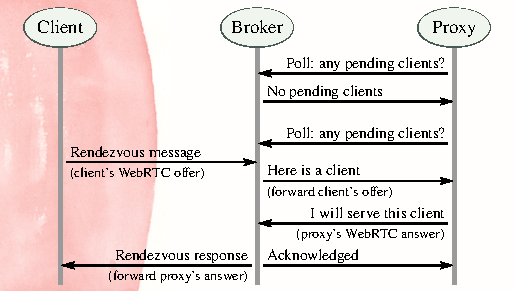
\includegraphics{figures/rendezvous/rendezvous}
\caption{
The long-polling communication model of Snowflake rendezvous.
Proxies poll periodically to check for new clients.
When the broker makes a match,
the proxy gets the client's SDP offer,
then immediately re-connects to send back its SDP answer.
It~all happens during one round trip from the client's perspective.
Not shown here is the indirect channel
used by the client to access the broker through the censor's zone of control
(shaded background).
}
\label{fig:rendezvous}
\todo[inline]{Replace provisional graphic.}
\end{figure}

The client needs to use an indirect channel,
resistant to blocking,
when communicating contacting the broker.
What is needed, essentially,
is a miniature circumvention system
to bootstrap into the full system.
What makes the rendezvous facet of circumvention
different from general circumvention
are its different, generally more lenient, requirements and assumptions,
which permit a larger solution space.
Because rendezvous accounts for only a small fraction
of total communication volume,
and it happens only infrequently,
it~can afford to use techniques that would be
too slow, expensive, or complicated
for real-time or bulk data transfer.
Another nice feature is that rendezvous is separable and modular:
more than one method can be used,
and the methods do not necessarily have to bear any relation
to the circumvention techniques of the main system.
While the assumption of WebRTC permeates Snowflake's design,
its rendezvous modules are independent.
We~currently support two rendezvous methods in Snowflake:

\begin{description}
\item[Domain fronting]
In~this method, the client does an HTTPS exchange with the broker
by an intermediary web service such as a CDN,
taking care to change the externally visible hostname
(the TLS Server Name Indication, or SNI)
from that of the broker to some other ``front domain''~\cite{Fifield2015a}.
The CDN routes the HTTPS request to the broker
according to the HTTP Host header, which remains unmodified
under the TLS encryption.
The well-known drawback of domain fronting
is the high financial cost of CDN bandwidth.
Because we use it only for rendezvous,
the cost is much more manageable than in a system
that uses domain fronting for all its data transfer.

% "AMP cache rendezvous" https://gitlab.torproject.org/tpo/anti-censorship/pluggable-transports/snowflake/-/merge_requests/50
\item[AMP cache]
AMP is a framework for web pages written in a restricted dialect of HTML.
Part of this framework is a free-to-use
cache server~\cite{amp-cache}.
The cache fetches origin web pages on demand,
which means that it is effectively as a restricted sort of HTTP proxy.
If~rendezvous messages are encoded to conform to AMP requirements,
they can be sent to the broker via the cache server.
Rendezvous through the AMP cache is not easily blocked
without blocking the cache server as a whole.
This rendezvous method still technically requires domain fronting,
because the AMP cache protocol would otherwise expose the
upstream server's hostname in the TLS SNI,
but it enlarges the set of usable intermediary web services and front domains.
\end{description}

Anything that can be persuaded to convey a rendezvous message
of about 1500 bytes indirectly to the broker,
and return a response of about the same size,
might work as a rendezvous module.
% "Broker: investigate non-domain-fronting secure client / proxy registrations" https://bugs.torproject.org/tpo/anti-censorship/pluggable-transports/snowflake/25594
For example, encrypted DNS
(DNS over TLS or DNS over HTTPS) would serve:
% "DNS-based rendezvous for Snowflake" https://bugs.torproject.org/tpo/anti-censorship/pluggable-transports/snowflake/25874
% \cite[\S 3.4]{Fifield2020a}
the client encodes its rendezvous message into a series of DNS queries
for hostnames whose authoritative resolver is the broker itself,
equipped with a module to reassemble the rendezvous message
and send a response in the form of DNS responses.
A~third-party recursive resolver acts as an intermediary for the broker,
while DNS encryption hides the broker's DNS zone from the censor.
% Flash proxy email rendezvous would not work for Snowflake, because unidirectional.
% https://gitweb.torproject.org/flashproxy.git/tree/flashproxy-reg-email
% https://gitweb.torproject.org/flashproxy.git/tree/facilitator/fp-registrar-email

Rendezvous is not unique to Snowflake.
Other examples of rendezvous in circumvention include
the DEFIANCE Rendezvous Protocol~\cite[\S 3]{Lincoln2012a},
the facilitator interaction in flash proxy~\cite[\S 3]{Fifield2012a},
and the registration proxy in Conjure~\cite[\S 4.1]{Frolov2019b}.
A~key property of rendezvous-based systems
is that they do not rely on preshared secret information.
The client needs only to acquire the necessary software;
whatever additional information is required to establish a circumvention session
is exchanged dynamically, at runtime.
A~corollary of the no-secret-information property
is that an adversary---the censor---is
at no special disadvantage in attacking the system.
The censor may download the client software,
run it, study its network connections,
and the system must remain blocking-resistant despite this.
This is in contrast to other systems in which,
in~addition to the necessary software,
a~client must acquire some secret,
such as a password or proxy IP address,
through an out-of-band channel
that is presumed to be unavailable to the censor,
and the system's blocking resistance depends on
clients keeping that information secret from the censor.
If~rendezvous has the advantage of not needing to manage secrets,
its disadvantage is that it just one more thing to get right.
Not only the main circumvention channel
but also the rendezvous must resist blocking:
the system is only as strong as the weaker of the~two.

\subsection{Peer-to-peer connection establishment}
\label{sec:ice}

Now the client and the proxy connect to each other directly.
Even in the absence of censorship,
making a direct connection between two Internet peers is not always easy,
because of NAT (network address translation) and firewalls.
Snowflake clients and proxies alike run in diverse networks
that have varying NATs and ingress policies.
Fortunately for us,
WebRTC is designed with this use case in mind,
and has built-in support for traversing NAT, namely
ICE (Interactive Connectivity Establishment)~\cite{rfc8445},
a procedure for testing candidate pairs of peer network addresses
to find a pair that works.
ICE~makes use of
STUN (Session Traversal Utilities for NAT)~\cite{rfc8489}
and third-party STUN servers that, among other services,
enable a host to learn its own external IP addresses.
The first part of ICE has already taken place at the beginning of rendezvous,
when the client and proxy contacted STUN servers to gather
external address candidates and included them in their respective
SDP offer and answer.

There is no guarantee that any two hosts will be able to make
a connection using the facilities of STUN alone.
Some address mapping and
filtering setups are simply incompatible.
In~the case of an incompatible pairing,
ICE would normally fall back to using
TURN (Traversal Using Relays around NAT)~\cite{rfc8656},
which is a kind of UDP proxy.
Such a fallback would be problematic for Snowflake,
because the TURN relays themselves
would become a focus of blocking by the censor.
% "Configure TURN servers for the proxy and/or client" https://bugs.torproject.org/tpo/anti-censorship/pluggable-transports/snowflake/25596
But Snowflake has an advantage most WebRTC applications do not.
Most WebRTC applications want to connect \emph{a particular} pair of peers,
whereas we are satisfied when a client can connect to \emph{any} proxy.
Snowflake clients and proxies self-assess their NAT type
and report it in interactions with the broker.
The broker takes NAT compatibility into account when matching
and avoids cases that would require a fallback to TURN.

% "Investigate Snowflake proxy failures" https://bugs.torproject.org/tpo/anti-censorship/pluggable-transports/snowflake/33666#note_2595319
% "Okay here's a summary of what I've found: ..."

Two factors are relevant
a Snowflake client or proxy's
ability to make a peer-to-peer connection:
how its NAT maps internal IP--port combinations to external ports,
and how its firewall filters incoming packets.
For our purposes, it suffices
to condense the combinations of NAT mapping and firewall filtering
into the following well-known NAT variations:

% https://datatracker.ietf.org/doc/html/rfc3489#section-5
\begin{description}
\item[Full cone]
The same internal IP--port pair always maps to the same external port.
Any remote host may send a packet to an internal IP address and port by sending a packet to the
mapped external port.
\item[Restricted cone]
Like full cone,
but incoming packets
are allowed only if
there has recently been an outgoing packet
to the same remote IP address.
\item[Port-restricted cone]
Like restricted cone,
but incoming packets are allowed only if
there has recently been an outgoing packet
to the same remote IP--port pair.
\item[Symmetric]
The external port depends on both
the internal IP--port pair and the remote IP--port pair.
Incoming packets are allowed only if
there has recently been an outgoing
packet to the same remote address.
\end{description}

\begin{table}
\definecolor{Ycolor}{Gray}{14}
\definecolor{ncolor}{Gray}{13}
\newcommand{\Y}{\cellcolor{Ycolor}\ding{51}}
\newcommand{\n}{\cellcolor{ncolor}--}
\newcommand{\rotlabel}[1]{\rotatebox{30}{#1}}
% \vphantom is to make the labels take up vertical space;
% \rlap is so they don't expand the horizontal size of table columns.
\newcommand{\rot}[1]{\vphantom{\rotlabel{#1}}\rotlabel{\rlap{#1}}}
\centering
\begin{tabular}{@{}rccccc@{\hspace{1.5ex}}l@{~}l@{}}
& % empty
\rot{No NAT} &
\rot{Full cone} &
\rot{Restricted cone} &
\rot{Port-restricted cone} &
\rot{Symmetric} &
&
\\
No NAT               & \Y & \Y & \Y & \Y & \Y & \multirow{3}{*}{\(\left.\rule[-12pt]{0pt}{24pt}\right\}\)} & \multirow{3}{*}{\footnotesize \makecell[l]{unrestricted \\proxy}} \\
Full cone            & \Y & \Y & \Y & \Y & \Y & \\
Restricted cone      & \Y & \Y & \Y & \Y & \Y & \\
Port-restricted cone & \Y & \Y & \Y & \Y & \n & \multirow{2}{*}{\(\left.\rule[-7pt]{0pt}{14pt}\right\}\)} & \multirow{2}{*}{\footnotesize \makecell[l]{restricted \\proxy}} \\
Symmetric            & \Y & \Y & \Y & \n & \n & \\
% \hfill hack to make \upbracefill work with colortbl:
% https://tex.stackexchange.com/questions/202138/upbracefill-filling-entire-tabular-cell-and-package-colortbl#comment474604_202143
                     & \multicolumn{4}{c}{\def\hfill{\hskip 0pt plus 1filll}\upbracefill} & \multicolumn{1}{c}{\clap{\footnotesize \def\hfill{\hskip 0pt plus 1filll}\upbracefill}} & \\
                     & \multicolumn{4}{c}{\footnotesize \makecell{unrestricted \\client}} & \multicolumn{1}{c}{\clap{\footnotesize \makecell{restricted \\client}}} \\
\end{tabular}
\caption{
Pairwise compatibility of NAT variants,
using the facilities of STUN alone
(no fallback to TURN).
The incompatible cases are when one peer's NAT is symmetric
and the other's is symmetric or port-restricted cone.
}
\label{tab:nat-matching}
\todo[inline]{Check style guide to see if caption should be before or after a table.}
\todo[inline]{Try to improve the alignment/appearance of braces.}
\end{table}

\autoref{tab:nat-matching}
shows the pairwise compatibility of NAT variations.
As~the incompatible cases always involve a symmetric NAT,
we further simplify matching by categorizing the variations into the types
\firstterm{unrestricted} (works with most other NATs) and
\firstterm{restricted} (works only with the more permissive NATs).
Unrestricted proxies may be matched with any client;
restricted proxies may be matched only with unrestricted clients.
The broker prefers to match unrestricted clients with restricted proxies,
% https://gitlab.torproject.org/tpo/anti-censorship/pluggable-transports/snowflake/-/blob/9edaee65470a1483bbdbe984e5e15a885f1e95d2/broker/ipc.go#L236
in~order to conserve unrestricted proxies
for the clients that need them.
Symmetric NAT is always considered restricted,
but port-restricted cone NAT is categorized differently
depending on the peer:
for proxies it is restricted, but
for clients it is unrestricted.
The asymmetric categorization is an approximation
to further help conserve unrestricted proxies
for clients with symmetric NATs.
Though it creates the potential for an incompatible match
between a symmetric proxy and a port-restricted cone client,
port-restricted cone proxies are common in practice,
and are compatible with port-restricted cone clients.
Our measurements show that clients with port-restricted cone NAT
can connect to around 80\%\todo{Measure that 80\% number again.}
of proxies considered restricted under this categorization.\todo{Does this mean 80\% of restricted proxies,
or 80\% of the time a client eventually gets a compatible proxy after repeated retries?}
In~case of a connection failure,
clients re-rendezvous and try again.

Clients and proxies self-assess their NAT type
and send it to the broker in their rendezvous messages.
Clients use the NAT behavior discovery feature of STUN~\cite{rfc5780}.
% "Use STUN to determine NAT behaviour of peers" https://bugs.torproject.org/tpo/anti-censorship/pluggable-transports/snowflake/34129
% "Add utility to help user discover their NAT type" https://github.com/pion/stun/issues/8
Not all STUN servers support NAT behavior discovery,
but those whose addresses we ship with the Snowflake client~do.
Proxies cannot use the same technique,
because the necessary STUN features are not available
to JavaScript code in web browsers.
% "Have a remote probe service to test snowflake proxy NAT compatability" https://bugs.torproject.org/tpo/anti-censorship/pluggable-transports/snowflake/40013
Instead
we adapt a technique from MassBrowser~\cite[\S \mbox{V-A}]{Nasr2020a}:
we~run a centralized, always-on WebRTC testing peer
behind a simulated symmetric NAT.
Proxies try to connect to this peer;
if~the connection succeeds, its type is unrestricted,
otherwise it is restricted.
Clients and proxies retest their NAT type periodically,
to account for potential changes in their local networking environment.
If~a client or proxy is unable to determine its NAT type for some reason,
it reports the type ``unknown,''
which the broker conservatively treats it as if it were restricted.

\begin{figure}
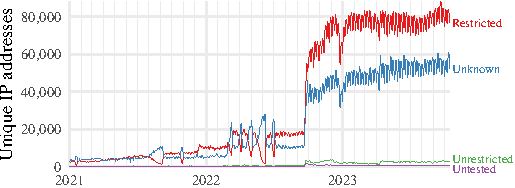
\includegraphics{figures/proxies/proxy-nat-type}
\caption{
Proxy NAT types, in unique IP addresses per day.
The places in 2021 and 2022
where there is an increase in the ``unknown'' NAT type
and a decrease in the other types
were the result of temporary operational problems with the
testing peer that proxies use to assess their NAT type.
% "Increase of 'unknown' NAT assignments by probetest since 2021-10-25" https://bugs.torproject.org/tpo/anti-censorship/pluggable-transports/snowflake/40071
% "Move snowflake-broker to a systemd based setup" https://bugs.torproject.org/tpo/anti-censorship/pluggable-transports/snowflake/40147
}
\label{fig:proxy-nat-type}
\end{figure}

\autoref{fig:proxy-nat-type}
shows that unrestricted proxies are
a relatively small fraction of the proxy population.
In~absolute terms, there are enough,
thanks in large part to the volunteers who run
the command-line
version of the Snowflake proxy
on networks unencumbered by NAT.
Though stable, long-term proxies are
against the ethos of Snowflake,
it~has proved useful, as a matter of practicality,
to~sacrifice a measure of address diversity
for better NAT compatibility in a common case.
Approximately one quarter of client polls
report a restricted NAT type.\todo{Double-check this number and document how it was calculated.}

At the same time as the proxy makes a connection to its assigned client,
% "At the same time": https://gitlab.torproject.org/tpo/anti-censorship/pluggable-transports/snowflake/40228
it also connects to the bridge.
For this connection we
use the WebSocket protocol~\cite{rfc6455}, which
offers a TCP-like, point-to-point, client--server connection
layered on HTTPS.
The choice of protocol for the proxy--bridge link is arbitrary,
and could be changed
without affecting the rest of the system.
The protocol does not need to be blocking-resistant;
it~just needs to be available to JavaScript code in web browsers.
WebRTC would serve for this link too.

\subsection{Data transfer}
\label{sec:data-transfer}

No~complicated processing takes place at the proxy.
The main value of a Snowflake proxy is its IP address:
it~gives the client a peer to connect to that is not on the censor's address blocklist.
Having provided that,
the proxy assumes a role of pure data transfer.

Snowflake uses a stack of nested protocol layers.
We~will walk though each layer and describe its purpose.

\bigskip

\noindent
\begin{tabular}{@{}l@{\,}l@{}l@{\,}l}
UDP & \rdelim\}{3}{*} & \multirow{3}{5em}{WebRTC data channel} & \rdelim\}{3}{*}[\,ephemeral, per proxy]\\
DTLS \\
SCTP \\
KCP & \rdelim\}{2}{*} & \multirow{2}{*}{Turbo Tunnel} & \rdelim\}{3}{*}[\,persistent, per session] \\
smux \\
\multicolumn{3}{@{}l}{Tor protocol} \\
\multicolumn{4}{@{}l}{application streams} \\
\end{tabular}

\bigskip

\noindent
This is the stack for the client--proxy link,
which is where WebRTC is used and which is
observed by the censor.
The stack for the proxy--bridge link is the same,
but with WebSocket in place of the
WebRTC data channel at the top.
The layers marked ``ephemeral'' are skimmed off
and replaced as proxies come and~go.
The layers marked ``persistent'' are instantiated once
in each circumvention session,
hold long-term state,
and are end-to-end between client and bridge.

The connection between a client and its proxy is
a WebRTC data channel~\cite{rfc8831},
which provides a way to send arbitrary binary messages between peers.
A~data channel is its own stack of three protocols:
UDP for network transport,
DTLS (Datagram TLS)
for confidentiality and integrity, and
SCTP (Stream Control Transmission Protocol)
for delimiting message boundaries
and other features like congestion control.
Working UDP port numbers will have been discovered
using ICE in the previous phase.
The peers authenticate one another
at the DTLS layer using certificate fingerprints
that were exchanged during rendezvous~\cite[\S 5.1]{rfc8842}.

Data channels are well-suited to Snowflake's needs.
(Circumvention is even one of the use cases listed in the specification~\cite[\S 3.2]{rfc8831}.)
But data channels are not the only option:
WebRTC also offers \firstterm{media streams}
for unreliable transport of real-time audio and video.
Which of these is used may be a fingerprinting vector.
We~will take up this topic in \autoref{sec:fingerprinting}.

If~clients only ever used one proxy,
the WebRTC data channel would be sufficient.
But a Snowflake proxy might
disappear at any moment,
and when that happens, its data channel goes with~it.
If~the client was in the middle of a long download,
for example, it should be possible to resume the download
without interruption after rendezvousing with a new proxy.
For this we need a shared notion of session state that exists
at the client and the bridge, not tied to any temporary proxy.
A~lack of session continuity across proxy failures
had been an unsolved problem in flash proxy~\cite[\S 5.2]{Fifield2012a}.

We~adopt the
Turbo Tunnel design pattern~\cite{Fifield2020a}
and insert a userspace
session and reliability protocol
between the ephemeral proxy data channels
and the client's own application streams.
% "[anti-censorship-team] Turbo Tunnel in Snowflake" https://lists.torproject.org/pipermail/anti-censorship-team/2020-February/000059.html
This part of the protocol stack
outlives any single proxy---it~belongs to
the client and the bridge.
Its critical function is to attach sequence numbers and acknowledgements
to packets of data---this
is how both ends know what parts of the data stream
need to be retransmitted after a temporary loss of proxy connectivity.
We~use a combination of
KCP~\cite{kcp} and
smux~\cite{smux}.
KCP provides reliability,
and smux detects the end of idle sessions and terminates them.
KCP and smux have shown their worth in other deployments,
and are easy to program,
but there is nothing about them on which we depend essentially.
Any other transport protocol that provides the necessary features
and can be implemented in userspace would~do,
such as QUIC, TCP, or (our own layer~of) SCTP.
We~prototyped successfully with QUIC before settling on KCP/\allowbreak smux.

% Not going to get into how we currently use reliable, ordered (TCP-like) data
% channels, but plan to switch to unreliable, unordered (UDP-like) data
% channels, a better fit for the underlying datagram-oriented Turbo Tunnel
% layer.
%
% "turn off reliable mode for WebRTC DataChannel" https://gitlab.torproject.org/tpo/anti-censorship/pluggable-transports/snowflake/-/merge_requests/109
% "Snowflake is currently using network resource in a so suboptimal way..." https://bugs.torproject.org/tpo/anti-censorship/pluggable-transports/snowflake/40251#note_2891751

Finally,
we must specify some concrete protocol
so that the client can tell the bridge
what remote destination to access on its behalf.
In~our deployment, this role is played by the Tor protocol.
After stripping away the WebRTC and Turbo Tunnel containers,
the Snowflake bridge feeds the client's data stream
into a local Tor bridge.
Almost anything would work here, with the caveat
that it should be end-to-end secure between the client and bridge,
to prevent inspection or tampering
by curious or malicious proxies---Snowflake proxies are ``untrusted messengers''
in the sense of
Feamster et~al.~\cite[\S 3]{Feamster2003a}.
Integration with Tor has the nice feature that
not even the Snowflake bridge is trusted
to see the plaintext or destination of client traffic,
let alone the temporary proxies.
Using Tor also has some drawbacks,
which we will comment on in
\autoref{sec:multi-bridge}
and
\autoref{sec:future}.

\section{Protocol fingerprinting}
\label{sec:fingerprinting}

% https://gitlab.torproject.org/tpo/anti-censorship/pluggable-transports/snowflake/-/wikis/Fingerprinting

Snowflake leans heavily into the ``address blocking'' side of circumvention,
but the ``content blocking'' part matters too.
The goal, as~always, is to make circumvention traffic
difficult to distinguish from other traffic the censor cares not to block.
Snowflake is inherently tied to WebRTC,
and can only be effective against a censor
that is not willing to block WebRTC protocols wholesale.
But even within that scope,
there are many variations in \emph{how}
WebRTC is implemented and used,
which, if~not carefully considered, might enable a censor
to selectively block only Snowflake,
while leaving other uses of WebRTC undisturbed.
Unfortunately for the circumvention developer,
the richness of WebRTC protocols
affords a large attack surface for fingerprinting.
Not only that, WebRTC leaves the details of
signaling---in~which peers exchange information
needed to set up a connection,
corresponding to Snowflake rendezvous---unspecified~\cite[\S 3]{rfc8825},
leaving every application to invent its own mechanism.
% "The choice of protocols for client-server and inter-server signaling, and the definition of the translation between them, are outside the scope of the WebRTC protocol suite described in this document."
% https://www.rfc-editor.org/rfc/rfc8829.html#section-3.1: "JSEP does not specify a particular signaling model or state machine, other than the generic need to exchange session descriptions in the fashion described by [RFC3264] (offer/answer)..."

As~WebRTC is designed for the web,
most implementations of WebRTC are embedded in web browsers,
and are not easily removed from that context.
Snowflake originally used a WebRTC library extracted from Chromium,
but that eventually proved unworkable for cross-platform deployment.
Since~2019, Snowflake has used Pion~\cite{pion-webrtc},
% "Evaluate pion WebRTC" https://bugs.torproject.org/tpo/anti-censorship/pluggable-transports/snowflake/28942
an independent implementation of WebRTC
not tied to any browser.
This is both good and bad.
The good is greater agility and less development friction,
and a working relationship with upstream developers
that enables us to get fingerprinting-related changes made;
we~would not be where we are today without~it.
The bad is that the WebRTC fingerprint of Pion
does not automatically match that of the mainly browser-originated
WebRTC that Snowflake aims to blend in with.

The following is a list of fingerprinting concerns
that bear on Snowflake, together with
how we have tried to address them.
The existence of a fingerprinting vulnerability
does not automatically invalidate a circumvention system:
censorship and circumvention are a dialog,
and even among demonstrable vulnerabilities,
some are more and some are less practical for a censor to take advantage~of.
The important thing is to have a solid foundation;
minor flaws may be patched up as necessary.

\begin{description}
\item[Selection of STUN servers]
It~is not unusual for a WebRTC application to use STUN,
but the choice of what STUN servers to use is up to the application.
Running dedicated STUN servers just for Snowflake would not work,
because a censor would experience no collateral harm in
simply blocking them by IP address.
Our deployment uses a pool of public STUN servers
that are used in applications other than circumvention,
filtered for those that support the NAT behavior discovery feature
described in \autoref{sec:ice}.
The client chooses a random subset of servers from the pool
when it makes a connection;
this is because not every STUN server is accessible
under every censor.
% I went to check stun.l.google.com for blocking in China,
% but OONI Probe does not measure that server as of v3.17.1:
% https://github.com/ooni/probe/issues/2417#issuecomment-1468478811

\item[Format of STUN messages]
STUN is most often deployed over plaintext UDP,
which leaves its messages open to inspection
and potential fingerprinting.
STUN messages consist of a fixed header
followed by a variable-length list of ordered
attributes~\cite[\S 5]{rfc8489}.
What attributes appear,
and their order,
depends on the STUN implementation
and how the application uses it.

We have not done anything in particular
to disguise STUN messages.
Though plaintext UDP is the most common,
STUN specifies other transports,
including encrypted ones like DTLS.
These may be options for Snowflake in the future---of~course,
only if they are common enough that their use
does not stick out on its own.
% "Investigate if STUN over TCP/TLS is beneficial to us" https://bugs.torproject.org/tpo/anti-censorship/pluggable-transports/snowflake/40240

\item[Rendezvous]
Because the rendezvous methods of
\autoref{sec:rendezvous}
are modular,
each one needs a separate justification
as to why it should be difficult to block.
Besides that, they must be implemented in a way
that does not expose accidental distinguishers.
For example, the domain fronting and AMP cache rendezvous methods
use HTTPS, which is TLS,
which means TLS fingerprinting is a concern~\cite[\S 5.1]{Fifield2015a}.
Snowflake, like many circumvention systems,
uses the uTLS package~\cite[\S VII]{Frolov2019a}
to get a client TLS fingerprint that is randomized or that imitates common browsers.
See \autoref{sec:block-ir} for an account of when
domain fronting rendezvous was briefly blocked in Iran,
because we were slow in activating uTLS.

Though each rendezvous method may be difficult to block in itself,
a~censor might combine a low-confidence detection of rendezvous
with features from other phases of the Snowflake data exchange
to strengthen its guess.

\item[DTLS]
The outermost layer of a WebRTC data connection,
the protocol directly exposed to a censor,
is DTLS (Datagram TLS) over UDP.
DTLS is an adaptation of TLS~\cite[\S 1]{rfc9147} to the datagram setting,
and therefore inherits the fingerprinting concerns of TLS~\cite{Frolov2019a}.
TLS/DTLS fingerprinting may involve, for example,
inspecting ClientHello messages to see what
ciphersuites and extensions are used,
and their order. It~may be that a certain combination
is specific to a particular implementation of a circumvention system,
and may therefore be blocked at low cost.

Due to practical considerations,
Snowflake's defenses to DTLS fingerprinting are not very robust,
and are reactive rather than proactive.
In~the realm of TLS one may use uTLS,
but there is as yet no equivalent of uTLS for DTLS.
The present way of altering DTLS fingerprints in Snowflake
is to submit a pull request upstream to Pion
whenever a fingerprint feature used for blocking is identified.
\autoref{sec:block-ru} documents how this has happened twice already,
in response to blocking in Russia.

% For reference, fingerprinting changes upstreamed to Pion:
% * IP addresses as SNI values
%   https://bugs.torproject.org/tpo/anti-censorship/pluggable-transports/snowflake/40014#note_2764715
%   https://github.com/pion/dtls/issues/406
%   https://github.com/pion/dtls/pull/407
% * supported_groups in Server Hello
%   https://bugs.torproject.org/tpo/anti-censorship/pluggable-transports/snowflake/40014#note_2765074
%   https://github.com/pion/dtls/issues/409
%   https://github.com/pion/dtls/pull/410
% * Server sending Hello Verify Request
%   https://bugs.torproject.org/tpo/anti-censorship/pluggable-transports/snowflake/40014#note_2764715
%   https://gitlab.torproject.org/tpo/applications/tor-browser-build/-/merge_requests/637
%   https://bugs.torproject.org/tpo/anti-censorship/pluggable-transports/snowflake/40249
%   https://github.com/pion/dtls/pull/513
%   https://github.com/pion/webrtc/pull/2407
%
% Not fingerprinting but also upstreamed:
% * NAT behavior detection
%   https://github.com/pion/stun/issues/8
%   https://github.com/pion/stun/pull/33

\item[Data channel or media stream]
Besides data channels, WebRTC offers \firstterm{media streams},
in line with its intended purpose of enabling real-time
audio and video communication.
Though both are encrypted,
data channels and media streams are externally distinguishable
because they use different containers.
Data channels use DTLS,
and media streams use DTLS-SRTP;
that is, the Secure Real-Time Transport Protocol
with a DTLS key exchange~\cite[\S 4.3]{rfc8827}.

Data channels are a closer match to Snowflake's communication model:
media streams are meant to contain encoded audio and video,
not arbitrary binary data.
But the use of DTLS rather than DTLS-SRTP could become
a significant feature if most other WebRTC applications use media streams.
Although it would be less convenient,
it would be possible to adapt the WebRTC link between
the client and its proxy
to use a media stream rather than a data channel,
either by modulating binary data into a well-formed encoded
audio or video signal in the manner of, say,
Stegozoa~\cite[\S 3.3]{Figueira2022a},
or by directly replacing the ciphertext of SRTP packets,
as in Protozoa~\cite[\S 4.4]{Barradas2020a}.
% See idea about WebRTC Encoded Transform: https://lists.torproject.org/pipermail/anti-censorship-team/2023-February/000284.html

\end{description}

Fifield and Gil Epner~\cite{arxiv.1605.08805}
studied the network traffic of WebRTC applications,
with the goal of revealing fingerprinting pitfalls
that might affect Snowflake, which was then in early development.
MacMillan et~al.~\cite{arxiv.2008.03254}
focused on the DTLS handshake,
comparing Snowflake to three other WebRTC applications.
They correctly anticipated features
of the Pion DTLS handshake
that would later actually be used
to block Snowflake in Russia;
see more details in \autoref{sec:block-ru}.

Chen et~al.~\cite{Chen2023a}
combined features
of rendezvous and DTLS
in order to reduce false positives.
Their classifier first prefilters
by looking for DNS queries for
STUN servers in the Snowflake client's default pool
and the default front domain used in
domain fronting rendezvous.
While a single DNS query is not strong evidence of Snowflake,
several related queries sent within a short time
are more deserving of attention.
They then apply a machine learning classifier
to features of any subsequent DTLS handshake.
The authors acknowledge that DTLS fingerprinting
is fragile, as the DTLS fingerprint is, in principle,
controllable by the application.
The DNS prefilter may perhaps be mitigated
by alternative rendezvous methods (\autoref{sec:rendezvous}),
or~by smarter selection of STUN servers by the client.

\begin{figure*}[t]
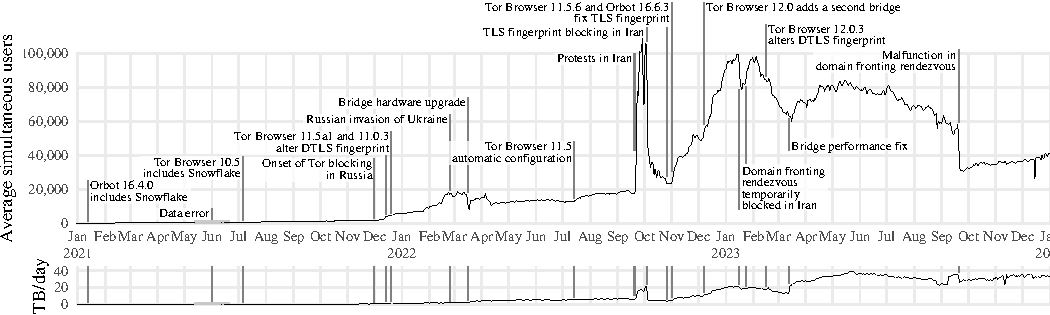
\includegraphics{figures/users/users-global}
\caption{
Estimated average simultaneous Snowflake users and bandwidth by day.
The values at the far left of the graph,
in~early January~2021, are about~60 users
% > filter(filtered, abs(date - as.Date("2021-01-01")) < 3)
% # A tibble: 5 x 3
%   date       transport users
%   <date>     <chr>     <dbl>
% 1 2020-12-30 snowflake  66.2
% 2 2020-12-31 snowflake  54
% 3 2021-01-01 snowflake  53.4
% 4 2021-01-02 snowflake  65.5
% 5 2021-01-03 snowflake  65.4
and 4~GB/day.
% > library("tidyverse")
% > WANTED_FINGERPRINTS <- c(
%     "7659DA0F96B156C322FBFF3ACCC9B9DC01C27C73" = "snowman",
%     "5481936581E23D2D178105D44DB6915AB06BFB7F" = "snowflake-01",
%     "91DA221A149007D0FD9E5515F5786C3DD07E4BB0" = "snowflake-02"
%   )
% > options(width = 200)
% > userstats <- read_csv("figures/users/userstats-bridge-transport-multi.csv") %>%
%     filter(fingerprint %in% names(WANTED_FINGERPRINTS)) %>%
%     mutate(users = users / (coverage / pmax(num_instances, coverage)))
% > bandwidth <- read_csv("figures/users/bandwidth-multi.csv") %>%
%     filter(fingerprint %in% names(WANTED_FINGERPRINTS)) %>%
%     filter(coverage > 0) %>%
%     mutate(bytes = bytes / (coverage / pmax(num_instances, coverage))) %>%
%     pivot_wider(id_cols = c(date, fingerprint), names_from = c(type), values_from = c(bytes)) %>%
%     mutate(
%       good_read = read - `dirreq-read`,
%       good_write = write - `dirreq-write`,
%       good_avg = (good_read + good_write) / 2
%     )
% > left_join(userstats, bandwidth, by = c("date", "fingerprint")) %>%
%     # Subtract out the pro-rated fraction of non-snowflake transports (basically negligible).
%     group_by(date, fingerprint) %>%
%     mutate(across(c(read, write, `dirreq-read`, `dirreq-write`, good_read, good_write, good_avg), ~ .x * users / sum(users))) %>%
%     ungroup() %>%
%     filter(transport == "snowflake") %>%
%     filter("2020-12-29" <= date & date < "2021-01-04") %>%
%     group_by(date) %>%
%     summarize(
%       date = last(date),
%       across(c(read, write, `dirreq-read`, `dirreq-write`, good_read, good_write, good_avg), sum, na.rm = TRUE)
%     ) %>%
%     mutate(across(c(read, write, `dirreq-read`, `dirreq-write`, good_read, good_write, good_avg), scales::label_bytes(units = "auto_si", accuracy = 0.01))) %>%
%     arrange(date) %>% tail()
% # A tibble: 6 × 8
%   date       read     write   `dirreq-read` `dirreq-write` good_read good_write good_avg
%   <date>     <chr>    <chr>   <chr>         <chr>          <chr>     <chr>      <chr>
% 1 2020-12-29 9.95 GB  8.89 GB 89.52 MB      825.81 MB      9.86 GB   8.07 GB    8.97 GB
% 2 2020-12-30 10.77 GB 9.07 GB 87.01 MB      787.05 MB      10.68 GB  8.28 GB    9.48 GB
% 3 2020-12-31 5.32 GB  5.13 GB 76.97 MB      682.87 MB      5.25 GB   4.45 GB    4.85 GB
% 4 2021-01-01 4.57 GB  4.25 GB 75.48 MB      683.19 MB      4.49 GB   3.57 GB    4.03 GB
% 5 2021-01-02 7.34 GB  6.56 GB 90.84 MB      822.81 MB      7.25 GB   5.74 GB    6.49 GB
% 6 2021-01-03 8.50 GB  7.74 GB 94.69 MB      844.65 MB      8.40 GB   6.90 GB    7.65 GB
}
\label{fig:user-counts}
\end{figure*}

\section{Experience}
\label{sec:experience}

Snowflake has now been in operation for a few years.
In~lieu of a forward-looking evaluation,
here we will take a look back
at the history of our deployment
and reflect on the experience.

\subsection{Client counts and bandwidth}
\label{sec:deployment}

% Excerpts from https://gitlab.torproject.org/tpo/network-health/metrics/timeline:
% |2017-01-24|||snowflake|Tor Browser 7.0a1 released, including Snowflake for GNU/Linux only.|[blog post](https://blog.torproject.org/blog/tor-browser-70a1-released)||
% |2017-08-08|||snowflake|Tor Browser 7.5a4 released, including Snowflake for macOS.|[blog post](https://blog.torproject.org/blog/tor-browser-75a4-released) [issue](https://bugs.torproject.org/tpo/applications/tor-browser/22831)||
% |2018-03-26 20:43:42|||snowflake|Release of Tor Browser 8.0a5. Improves snowflake client performance.|[blog post](https://blog.torproject.org/tor-browser-80a5-released) [ticket](https://bugs.torproject.org/tpo/anti-censorship/pluggable-transports/snowflake/21312)||
% |2019-10-01|||snowflake|Release of Tor Browser 9.0a7, the first release that has Snowflake for Windows.|[blog post](https://blog.torproject.org/new-release-tor-browser-90a7) [ticket](https://bugs.torproject.org/tpo/anti-censorship/pluggable-transports/snowflake/25483)||
% |2020-05-22 19:51:29|||snowflake|Release of Tor Browser 9.5a13, the first release with Turbo Tunnel session persistence features for Snowflake. There is a spike in estimated users on 2020-05-21 and 2020-05-22, which appears to be an artifact.|[blog post](https://blog.torproject.org/new-release-tor-browser-95a13) [ticket](https://bugs.torproject.org/tpo/applications/tor-browser/34043) [users graph](https://metrics.torproject.org/userstats-bridge-transport.html?start=2020-03-01&end=2020-08-01&transport=snowflake)||
% |2020-06-02 18:09:48|||snowflake|Release of Tor Browser 10.0a1, the first release with Snowflake for Android.|[blog post](https://blog.torproject.org/new-release-tor-browser-100a1) [ticket](https://bugs.torproject.org/tpo/applications/tor-browser/30318)||
% |2020-06-25|2020-06-25||snowflake|One- or two-day spike in estimated Snowflake users. It resembles the spike that occurred around the time of the Turbo Tunnel release of Tor Browser 9.5a13 on 2020-05-22.|[users graph](https://metrics.torproject.org/userstats-bridge-transport.html?start=2020-03-01&end=2020-08-01&transport=snowflake)|X|
% |2020-08-19|||snowflake|Release of Tor Browser 10.0a5, which added added the ability to do NAT behavior discovery to the Snowflake client.|[blog post](https://blog.torproject.org/new-release-tor-browser-100a5/) [issue](https://bugs.torproject.org/tpo/applications/tor-browser-build/40016)||
% |2020-10-29|||snowflake|Release of Snowflake WebExtension 0.5.0, with a NAT type self-test.|[archive](https://archive.org/details/snowflake-webextension-0.5.0) [issue](https://bugs.torproject.org/tpo/anti-censorship/pluggable-transports/snowflake/40013)||
% |2020-11-17|||snowflake|Release of Snowflake WebExtension 0.5.2, with a fix to the NAT type self-test.|[archive](https://archive.org/details/snowflake-webextension-0.5.2) [merge request](https://gitlab.torproject.org/tpo/anti-censorship/pluggable-transports/snowflake-webext/-/merge_requests/9) [comment](https://bugs.torproject.org/tpo/anti-censorship/pluggable-transports/snowflake/40013#note_2716071)||
% |2021-01-12|||snowflake|Release of Orbot 16.4.0-RC-1-tor-0.4.4.6, first release with Snowflake client support.|[release](https://github.com/guardianproject/orbot/releases/tag/16.4.0-RC-1-tor-0.4.4.6)||
% |2021-02-23|||snowflake|Release of Orbot 16.4.1-BETA-2-tor.0.4.4.6, with experimental Snowflake proxy support.|[release](https://github.com/guardianproject/orbot/releases/tag/16.4.1-BETA-2-tor.0.4.4.6)||
% |2021-07-06 16:56:37|||snowflake|Release of Tor Browser 10.5, first stable release that includes Snowflake.|[blog post](https://blog.torproject.org/new-release-tor-browser-105)||
% |2021-12-01|ongoing|ru||Blocking of Tor directory authorities, relays, default obfs4 bridges, meek-azure, and Snowflake in some ISPs in Russia. There was a temporary cease of blocking for less than a day starting on 2021-12-08.|[NTC thread](https://ntc.party/t/ooni-reports-of-tor-blocking-in-certain-isps-since-2021-12-01/1477) [BBS thread](https://github.com/net4people/bbs/issues/97) [issue](https://bugs.torproject.org/tpo/community/support/40050) [blog post](https://blog.torproject.org/tor-censorship-in-russia/) [OONI report](https://ooni.org/post/2021-russia-blocks-tor/#blocking-of-the-tor-network)||
% |2021-12-14|||snowflake|Release of Tor Browser 11.5a1, with an altered DTLS fingerprint in Snowflake to counteract blocking in Russia.|[blog post](https://blog.torproject.org/new-release-tor-browser-115a1/) [issue](https://bugs.torproject.org/tpo/applications/tor-browser-build/40393) [NTC post](https://ntc.party/t/ooni-reports-of-tor-blocking-in-certain-isps-since-2021-12-01/1477/59)||
% |2021-12-20|||snowflake|Release of Tor Browser 11.0.3, with an altered DTLS fingerprint in Snowflake to counteract blocking in Russia.|[blog post](https://blog.torproject.org/new-release-tor-browser-1103/) [issue](https://bugs.torproject.org/tpo/applications/tor-browser-build/40393) [NTC post](https://ntc.party/t/ooni-reports-of-tor-blocking-in-certain-isps-since-2021-12-01/1477/59)||
% |2022-01-25 17:41:00|||snowflake|Switched the snowflake bridge to a temporary load-balanced staging server. Debugged connection problems until 2022-01-25 18:47:00.|[issue](https://bugs.torproject.org/tpo/tpa/team/40598#note_2772287) [comment](https://bugs.torproject.org/tpo/anti-censorship/pluggable-transports/snowflake/40095#note_2772325) [post](https://forum.torproject.net/t/tor-relays-how-to-reduce-tor-cpu-load-on-a-single-bridge/1483/16) [comment](https://github.com/net4people/bbs/issues/103#issuecomment-1033067920)||
% |2022-03-16 16:51:35|||snowflake|Moved Snowflake traffic to the interim bridge running instances flakey1–flakey8.|[comment](https://bugs.torproject.org/tpo/tpa/team/40664#note_2787624)||
% |2022-05-06 12:14:51|||snowflake|Upgraded the network uplink of the Snowflake bridge from 1 Gbps to 10 Gbps.|[issue](https://bugs.torproject.org/tpo/anti-censorship/pluggable-transports/snowflake/40138)||
% |2022-06-27|||snowflake|Deployed version 0.6.0 of the Snowflake WebExtension. The main feature added in this release was support for more than one bridge. It had a bug that caused it to stop reporting client IP addresses, which are used for metrics purposes by the bridge.|[archive](https://archive.org/details/snowflake-webextension-0.6.0) [merge request](https://gitlab.torproject.org/tpo/anti-censorship/pluggable-transports/snowflake-webext/-/merge_requests/29) [issue](https://bugs.torproject.org/tpo/anti-censorship/pluggable-transports/snowflake-webext/82)||
% |2022-07-14|||bridge|Release of Tor Browser 11.5, with a new feature of automatic censorship circumvention configuration.|[blog post](https://blog.torproject.org/new-release-tor-browser-115/)||
% |2022-09-21|ongoing|ir||Protests and daily Internet shutdowns in Iran.|[OONI report](https://ooni.org/post/2022-iran-blocks-social-media-mahsa-amini-protests/) [BBS thread](https://github.com/net4people/bbs/issues/125)||
% |2022-10-03 12:50:34|||snowflake|Deployment of Snowflake broker to reject proxies that do not support multiple bridges.|[issue](https://bugs.torproject.org/tpo/anti-censorship/pluggable-transports/snowflake/40193) [issue](https://bugs.torproject.org/tpo/anti-censorship/team/95)||
% |2022-10-04 17:15:00|||snowflake|Snowflake rendezvous blocked by TLS fingerprint in Iran.|[issue](https://bugs.torproject.org/tpo/anti-censorship/pluggable-transports/snowflake/40207) [BBS thread](https://github.com/net4people/bbs/issues/131)||
% |2022-10-12|||snowflake|Release of Tor Browser 11.5.4. Adds uTLS TLS camouflage support for Snowflake, making a manual configuration possible to circumvent recent TLS blocking in Iran.|[blog post](https://blog.torproject.org/new-release-tor-browser-1154/) [BBS comment](https://github.com/net4people/bbs/issues/131#issuecomment-1280391051)||
% |2022-10-17 15:52:00||ir|snowflake|Enabled uTLS for Snowflake in Iran in the Circumvention Settings API, using the `hellochrome_auto` fingerprint.|[comment](https://bugs.torproject.org/tpo/anti-censorship/team/96#note_2844378) [merge request](https://gitlab.torproject.org/tpo/anti-censorship/rdsys-admin/-/merge_requests/6)||
% |2022-10-20 15:16:00|||snowflake|Release of Orbot for Android 16.6.3-BETA-2-tor.0.4.7.10. Adds uTLS TLS camouflage support for Snowflake, making it possible to circumvent recent TLS blocking in Iran.|[release](https://github.com/guardianproject/orbot/releases/tag/16.6.3-BETA-2-tor.0.4.7.10) [announcement](https://github.com/net4people/bbs/issues/125#issuecomment-1285897627)||
% |2022-10-27|||snowflake|Release of Tor Browser 11.5.6. Fixes the problem that prevented Snowflake from working in 11.5.5, and enables uTLS TLS camouflage support by default for Snowflake.|[blog post](https://blog.torproject.org/new-release-tor-browser-1156/) [issue](https://bugs.torproject.org/tpo/applications/tor-browser-build/40665)||
% |2022-11-01||ir|snowflake|Orbot begins a gradual release rollout of version 16.6.3-RC-1-tor.0.4.7.10, which has TLS fingerprint changes to make Snowflake work in Iran again.|[release](https://github.com/guardianproject/orbot/releases/tag/16.6.3-RC-1-tor.0.4.7.10)||
% |2022-12-01|||snowflake|Release of Tor Browser 12.0a5, the first release to contain both the snowflake-01 and snowflake-02 bridges.|[issue](https://bugs.torproject.org/tpo/applications/tor-browser-build/40674) [announcement](https://lists.torproject.org/pipermail/tor-announce/2022-December/000256.html) [BBS comment](https://github.com/net4people/bbs/issues/152#issuecomment-1336220171)||
% |2022-12-07|||snowflake|Release of Tor Browser 12.0, the first stable release to contain both the snowflake-01 and snowflake-02 bridges.|[issue](https://bugs.torproject.org/tpo/applications/tor-browser-build/40674) [blog post](https://blog.torproject.org/new-release-tor-browser-120/) [BBS comment](https://github.com/net4people/bbs/issues/152#issuecomment-1342800169) [NTC comment](https://ntc.party/t/second-snowflake-bridge-available-for-testing/3445/2)||
% |2023-01-16|2023-01-24|ir|moat snowflake|The domain name cdn.sstatic.net, which is used by Snowflake and Moat, is blocked in some ISPs in Iran.|[comment](https://bugs.torproject.org/tpo/anti-censorship/team/115#note_2873040)||
% |2023-01-31|2023-02-01|ir|moat snowflake|The domain name cdn.sstatic.net, which is used by Snowflake and Moat, is again blocked in some ISPs in Iran.|[comment](https://bugs.torproject.org/tpo/anti-censorship/team/115#note_2876012)||
% |2023-02-08|2023-02-13|ir|moat snowflake|The domain name cdn.sstatic.net, which is used by Snowflake and Moat, is again blocked in some ISPs in Iran.|[comment](https://bugs.torproject.org/tpo/anti-censorship/team/115#note_2883298) [OONI chart](https://explorer.ooni.org/chart/mat?probe_cc=IR&since=2023-01-23&until=2023-03-01&time_grain=day&axis_x=measurement_start_day&test_name=web_connectivity&domain=cdn.sstatic.net)||
% |2023-02-15|||snowflake|Release of Tor Browser 12.0.3. Has a change to the Snowflake DTLS fingerprint (removes Hello Verify Request) to mitigate reported blocking in Russia.|[blog post](https://blog.torproject.org/new-release-tor-browser-1203/) [comment about Hello Verify Request](https://bugs.torproject.org/tpo/anti-censorship/censorship-analysis/40030#note_2823140) [Snowflake merge request](https://gitlab.torproject.org/tpo/anti-censorship/pluggable-transports/snowflake/-/merge_requests/134) [Tor Browser merge request](https://gitlab.torproject.org/tpo/applications/tor-browser-build/-/merge_requests/637)||
% |2023-02-19|2023-02-19|ir|moat snowflake|The domain name cdn.sstatic.net, which is used by Snowflake and Moat, is again blocked in some ISPs in Iran.|[comment](https://bugs.torproject.org/tpo/anti-censorship/team/115#note_2883298) [OONI chart](https://explorer.ooni.org/chart/mat?probe_cc=IR&since=2023-01-23&until=2023-03-01&time_grain=day&axis_x=measurement_start_day&test_name=web_connectivity&domain=cdn.sstatic.net)||
% |2023-02-22|2023-02-22|ir|moat snowflake|The domain name cdn.sstatic.net, which is used by Snowflake and Moat, is again blocked in some ISPs in Iran.|[comment](https://bugs.torproject.org/tpo/anti-censorship/team/115#note_2883298) [OONI chart](https://explorer.ooni.org/chart/mat?probe_cc=IR&since=2023-01-23&until=2023-03-01&time_grain=day&axis_x=measurement_start_day&test_name=web_connectivity&domain=cdn.sstatic.net)||
% |2023-03-13 19:46:07|||snowflake|Restarted snowflake-02 bridge for a bugfix.|[comment](https://bugs.torproject.org/tpo/anti-censorship/pluggable-transports/snowflake/40262#note_2886032) [issue](https://bugs.torproject.org/tpo/anti-censorship/pluggable-transports/snowflake/40260)||
% |2023-03-13 20:17:54|||snowflake|Restarted snowflake-01 bridge for a bugfix.|[comment](https://bugs.torproject.org/tpo/anti-censorship/pluggable-transports/snowflake/40262#note_2886041) [issue](https://bugs.torproject.org/tpo/anti-censorship/pluggable-transports/snowflake/40260)||
% |2023-03-15|||snowflake|Release of Orbot for Android v17 BETA 2. First release of Orbot to include the snowflake-02 bridge along with the existing snowflake-01. Has a change to the Snowflake DTLS fingerprint (removes Hello Verify Request) to mitigate reported blocking in Russia.|[release](https://github.com/guardianproject/orbot/releases/tag/17.0.0-BETA-2-tor.0.4.7.11) [Orbot commit adding snowflake-02](https://github.com/guardianproject/orbot/commit/c3f6ee18f17770a5904ad19c3cd24b9c8dcb3885) [IPtProxy commit upgrading Snowflake](https://github.com/tladesignz/IPtProxy/commit/5d0654a6a1439c05d3ee52b2b351b5df1ff3f6dc)||

Snowflake became available to end users gradually,
reflecting a long development process.
Deployment began in~2017,
but the system only really became usable in~2020.
It~began to attract large numbers of users
(enough to merit a censor's attention)
in~2022, following generalized
network blocking events in Russia and Iran.

Snowflake shipped in the alpha release series of Tor Browser
before graduating to the stable series.
It~was first released for GNU/Linux
in Tor Browser~7.0a1 on \mbox{2017-01-24},
% "First working bundles with Snowflake, for linux only" https://bugs.torproject.org/tpo/anti-censorship/pluggable-transports/snowflake/19001
% "Add snowflake pt to alpha linux builds" https://bugs.torproject.org/tpo/applications/tor-browser/20735
and for macOS
in Tor Browser~7.5a4 on \mbox{2017-08-08}.
% "mac reproducible build" https://bugs.torproject.org/tpo/anti-censorship/pluggable-transports/snowflake/19001
% "[tbb-dev] Please check reproducibility of mac build with Snowflake (e084e83418)" https://lists.torproject.org/pipermail/tbb-dev/2017-July/000579.html
% "Merge Snowflake for mac" https://bugs.torproject.org/tpo/applications/tor-browser/22831
But we hit a roadblock in attempting to prepare releases for other platforms:
the Chromium-derived WebRTC library we had used to that point
presented major difficulties
in Tor Browser's
cross-compiling, reproducible build environment.
What let us resume making progress was a switch to
Pion WebRTC~\cite{pion-webrtc} in~2019.
With it, we~were able to release
Snowflake for Windows
in Tor Browser~9.0a7 on \mbox{2019-10-01},
% "Android reproducible build of Snowflake" https://bugs.torproject.org/tpo/applications/tor-browser/28672
% "Integrate snowflake into mobile Tor Browser alpha" https://bugs.torproject.org/tpo/applications/tor-browser/30318
and for Android in
Tor Browser~10.0a1 on \mbox{2020-06-02}.

While at this point Snowflake was available
on every platform supported by Tor Browser,
it was not yet comfortably usable.
There were two important parts missing:
no NAT type matching (\autoref{sec:ice})
meant that a client could not always connect to its assigned proxy;
and a lack of persistent session state (\autoref{sec:data-transfer})
meant that even if a proxy connection was successful,
the client's session would end once that proxy disappeared.
For these reasons, by early 2020,
the average number of concurrent users
had not risen above~40.
% > library("tidyverse")
% > WANTED_FINGERPRINTS <- c(
%     "7659DA0F96B156C322FBFF3ACCC9B9DC01C27C73" = "snowman",
%     "5481936581E23D2D178105D44DB6915AB06BFB7F" = "snowflake-01",
%     "91DA221A149007D0FD9E5515F5786C3DD07E4BB0" = "snowflake-02"
%   )
% > userstats <- read_csv("figures/users/userstats-bridge-transport-multi.csv") %>%
%     filter(transport == "snowflake" & fingerprint %in% names(WANTED_FINGERPRINTS)) %>%
%     mutate(users = users / (coverage / pmax(num_instances, coverage))) %>%
%     group_by(date, transport) %>% summarize(users = sum(users, na.rm = TRUE), .groups = "drop")
%
% Ignoring two apparently anomalous spikes before 2021.
% One on 2020-05-21 and 2020-05-22 (the day of the Turbo Tunnel release):
% > filter(userstats, "2020-05-19" <= date & date <= "2020-05-24")
% # A tibble: 6 x 3
%   date       transport  users
%   <date>     <chr>      <dbl>
% 1 2020-05-19 snowflake   9.16
% 2 2020-05-20 snowflake  14.7
% 3 2020-05-21 snowflake 133.
% 4 2020-05-22 snowflake 388.
% 5 2020-05-23 snowflake   7.9
% 6 2020-05-24 snowflake  13.9
% One on 2020-06-25 and 2020-06-26 (not sure what this one is about):
% > filter(userstats, "2020-06-23" <= date & date <= "2020-06-28")
% # A tibble: 6 x 3
%   date       transport users
%   <date>     <chr>     <dbl>
% 1 2020-06-23 snowflake  17.0
% 2 2020-06-24 snowflake  20.2
% 3 2020-06-25 snowflake  71.7
% 4 2020-06-26 snowflake 211.
% 5 2020-06-27 snowflake  22.5
% 6 2020-06-28 snowflake  33.7
%
% > filtered <- filter(userstats, !(date %in% as.Date(c("2020-05-21", "2020-05-22", "2020-06-25", "2020-06-26"))))
% > filtered[which.max(filter(filtered, date < "2020-05-21")$users), ]
% # A tibble: 1 x 3
%   date       transport users
%   <date>     <chr>     <dbl>
% 1 2020-04-01 snowflake  34.0
The Turbo Tunnel session persistence feature
became available to users in Tor Browser~9.5a13
on \mbox{2020-05-22}.
% "Merge a turbotunnel branch" https://bugs.torproject.org/tpo/anti-censorship/pluggable-transports/snowflake/33745
% "Update snowflake to persist sessions across proxies" https://bugs.torproject.org/tpo/applications/tor-browser/34043
The client part of NAT behavior detection
was released with Tor Browser~10.0a5 on \mbox{2020-08-19},
% "Use STUN to determine NAT behaviour of peers" https://bugs.torproject.org/tpo/anti-censorship/pluggable-transports/snowflake/34129
% "Update snowflake version and prefs to do nat discovery at the client" https://bugs.torproject.org/tpo/applications/tor-browser-build/40016
and the necessary proxy support was added on \mbox{2020-11-17}.
% "Have a remote probe service to test snowflake proxy NAT compatability" https://bugs.torproject.org/tpo/anti-censorship/pluggable-transports/snowflake/40013
% "Wait for ice gathering to complete before probtest" https://gitlab.torproject.org/tpo/anti-censorship/pluggable-transports/snowflake-webext/-/merge_requests/9
% "after merging snowflake-webext!9 (merged), this is finally working" https://bugs.torproject.org/tpo/anti-censorship/pluggable-transports/snowflake/40013#note_2716071
% https://archive.org/details/snowflake-webextension-0.5.2
After these changes, Snowflake became practical for daily browsing
and the number of users began to grow into~2021.

This bring us to \autoref{fig:user-counts}, which
shows the number of Snowflake users since 2021.
The number of users is estimated using the aggregate statistics
reported by the Tor bridge
and the formulas of Tor Metrics~\cite{tor-tr-2012-10-001}.
Tor Metrics graphs are frequently misinterpreted.
Be aware: the chart does not show a count of unique clients,
but rather the \emph{average number of concurrent clients} per day.
% "The result is an average number of concurrent users, estimated from data collected over a day. We can't say how many distinct users there are."
% https://metrics.torproject.org/reproducible-metrics.html#users
% $ grep '^2022-05-01.*,snowflake,' figures/users/userstats-bridge-transport-multi.csv
% 2022-05-01,5481936581E23D2D178105D44DB6915AB06BFB7F,snowflake,12235.62,100.00
For example, the value of 12,000 on \mbox{2022-05-01}
means that, on~average, 12,000 clients were using the service
at any point in time on that day.
The contribution of a client is independent of
the number of temporary proxies it uses
over the course of a session.

Snowflake's growth began in earnest
when it became part of default installations.
Orbot, a mobile app that provides a VPN-like Tor proxy,
added a Snowflake client in version 16.4.0
on \mbox{2021-01-12}.
% https://github.com/guardianproject/orbot/releases/tag/16.4.0-RC-1-tor-0.4.4.6 2021-01-12
% https://github.com/guardianproject/orbot/blob/a69f39bb37469e65730d0751519848ec29001959/CHANGELOG#L788 /** 16.4.0-RC-1-tor-0.4.4.6 / 12 January 2021 **/
% https://lists.mayfirst.org/pipermail/guardian-dev/2023-July/005704.html
Snowflake graduated to Tor Browser's stable series
in Tor Browser~10.5
on \mbox{2021-07-06},
% https://blog.torproject.org/new-release-tor-browser-105
becoming a third built-in circumvention option
alongside meek and obfs4.
% https://gitlab.torproject.org/tpo/applications/tor-browser-build/-/blob/tbb-10.5-build1/projects/tor-browser/Bundle-Data/PTConfigs/bridge_prefs.js
Being part of a stable release meant that it was
easily available to all Tor users,
not a self-selected group of alpha users.
The number of users steadily increased
over the next five months,
reaching almost~2,000 by December~2021.

Network censorship events may have the contrary effects
of either increasing or decreasing the number of users
of a circumvention system.
The user count will decrease
if the system does not have enough resistance to prevent
itself being caught up in the blocking;
but increase if it remains unblocked as one
of a diminished number of ways to reach the outside world.
Two such censorship events,
one in Russia and one in Iran,
had the effect of increasing the number of Snowflake users
by multiples.
(Because they also, in part, threatened Snowflake itself,
we will have more to say about them in \autoref{sec:block}.)

On \mbox{2021-12-01}, some ISPs in Russia
deployed measures to block
most forms of access to Tor,
including Snowflake~\cite{ooni-2021-russia-blocks-tor}.
The measures varied in their effectiveness;
in~the case of Snowflake,
blocking was triggered by a particular feature of the DTLS handshake,
which we were able to mitigate in new releases within a few weeks.
Over the next two months the total number of Snowflake users quadrupled,
with most of the new users coming from Russia.
The sudden demand temporarily overwhelmed the bridge, and
for a few weeks Snowflake was almost unusably slow.
% "I really want to use snowflake, but it's extremely slow, almost unusable." https://old.reddit.com/r/TOR/comments/t49i14/hello_i_have_a_problem_with_snowflake_can_you/
It~forced us to rearchitect the bridge for better scaling~\cite{Fifield2023a},
% https://forum.torproject.net/t/tor-relays-how-to-reduce-tor-cpu-load-on-a-single-bridge/1483
% "The DNS records were changed to point to the staging bridge at..." https://bugs.torproject.org/tpo/anti-censorship/pluggable-transports/snowflake/40095#note_2772325
as~well as move the bridge to a powerful dedicated server
and upgrade its network link from 1~Gbps to 10~Gbps.
% https://forum.torproject.net/t/tor-project-more-resources-required-for-snowflake-bridge/2353
% "snowflake-01: Change uplink from 1G to 10G" https://bugs.torproject.org/tpo/anti-censorship/pluggable-transports/snowflake/40138
By~May 2022,
about 70\% of Snowflake users were in Russia.
% > library("tidyverse")
% > WANTED_FINGERPRINTS <- c(
%     "7659DA0F96B156C322FBFF3ACCC9B9DC01C27C73" = "snowman",
%     "5481936581E23D2D178105D44DB6915AB06BFB7F" = "snowflake-01",
%     "91DA221A149007D0FD9E5515F5786C3DD07E4BB0" = "snowflake-02"
%   )
% > userstats <- read_csv("figures/users/userstats-bridge-combined-multi.csv") %>%
%     filter(transport == "snowflake" & fingerprint %in% names(WANTED_FINGERPRINTS)) %>%
%     mutate(across(c(low, high), ~ .x / (coverage / pmax(num_instances, coverage)))) %>%
%     mutate(users = (low + high) / 2) %>%
%     # Combine the contributions of all bridges.
%     group_by(date, transport, country) %>% summarize(across(c(low, high, users), sum), .groups = "drop") %>%
%     # Apportion "??" to other countries (see figures/users/users-country.r).
%     group_by(date, transport) %>% mutate(across(c(low, high, users), ~ .x * sum(.x) / sum(ifelse(country == "??", 0, .x)))) %>% ungroup() %>% filter(country != "??")
% > userstats %>% filter(date == "2022-05-20") %>% arrange(desc(users)) %>%
%     mutate(percent = users / sum(users) * 100) %>% head()
% # A tibble: 6 x 7
%   date       transport country   low  high users percent
%   <date>     <chr>     <chr>   <dbl> <dbl> <dbl>   <dbl>
% 1 2022-05-20 snowflake ru      9311. 9311. 9311.   70.4
% 2 2022-05-20 snowflake us      1108. 1109. 1109.    8.38
% 3 2022-05-20 snowflake cn       533.  535.  534.    4.04
% 4 2022-05-20 snowflake de       256.  258.  257.    1.94
% 5 2022-05-20 snowflake by       200.  202.  201.    1.52
% 6 2022-05-20 snowflake gb       184.  186.  185.    1.40
The count of users in Russia got an additional small boost,
visible in the graph,
starting on \mbox{2022-07-14},
when Tor Browser~11.5 added the Connection Assist feature,
which automatically enables circumvention options when needed.
% https://blog.torproject.org/new-release-tor-browser-115/
% Graph showing boost going mostly to Russia: https://bugs.torproject.org/tpo/anti-censorship/pluggable-transports/snowflake-webext/82#note_2891387
Another DTLS blocking signature was reported on \mbox{2022-06-20};
we did not get to fixing it until Tor Browser~12.0.3 on \mbox{2023-02-15}.\todo{And Orbot 17 on\ldots}
% "The 'skip Hello Verify Request' change was merged into Tor Browser..." https://gitlab.torproject.org/tpo/anti-censorship/censorship-analysis/-/issues/40030#note_2893870
By~that time the global user count had come to be dominated by users from Iran.

% "Shutdowns, intensified blocking in Iran since 2022-09-21" https://github.com/net4people/bbs/issues/125
% "Need to increase number of tor instances on snowflake-01 bridge, increased usage since yesterday [2022-09-21]" https://lists.torproject.org/pipermail/anti-censorship-team/2022-September/000247.html
% "Graphs of user counts from Iran since the onset of shutdowns" https://forum.torproject.net/t/graphs-of-user-counts-from-iran-since-the-onset-of-shutdowns/4843
The next event that had a large effect on Snowflake usage
were the nationwide protests in Iran that started on \mbox{2022-09-21}.
The government imposed periodic network shutdowns
and additional network blocking,
severe even by the standards of a country already notorious
for Internet censorship~\cite{ooni-2022-iran-blocks-social-media-mahsa-amini-protests}.
Internet users in Iran turned to circumvention systems
that continued working despite the new restrictions,
Snowflake among them.
Adoption was rapid:
on~\mbox{2022-09-20}, Iran accounted for only~1\% of Snowflake users;
on~\mbox{2022-09-24} it was 67\%.
% > library("tidyverse")
% > WANTED_FINGERPRINTS <- c(
%     "7659DA0F96B156C322FBFF3ACCC9B9DC01C27C73" = "snowman",
%     "5481936581E23D2D178105D44DB6915AB06BFB7F" = "snowflake-01",
%     "91DA221A149007D0FD9E5515F5786C3DD07E4BB0" = "snowflake-02"
%   )
% > userstats <- read_csv("figures/users/userstats-bridge-combined-multi.csv") %>%
%     filter(transport == "snowflake" & fingerprint %in% names(WANTED_FINGERPRINTS)) %>%
%     mutate(across(c(low, high), ~ .x / (coverage / pmax(num_instances, coverage)))) %>%
%     mutate(users = (low + high) / 2) %>%
%     # Combine the contributions of all bridges.
%     group_by(date, transport, country) %>% summarize(across(c(low, high, users), sum), .groups = "drop") %>%
%     # Apportion "??" to other countries (see figures/users/users-country.r).
%     group_by(date, transport) %>% mutate(across(c(low, high, users), ~ .x * sum(.x) / sum(ifelse(country == "??", 0, .x)))) %>% ungroup() %>% filter(country != "??")
% > userstats %>% filter("2022-09-19" <= date & date <= "2022-09-25") %>%
%     group_by(date, transport) %>% mutate(percent = users / sum(users) * 100) %>% filter(country == "ir") %>% ungroup()
% # A tibble: 7 x 7
%   date       transport country    low   high  users percent
%   <date>     <chr>     <chr>    <dbl>  <dbl>  <dbl>   <dbl>
% 1 2022-09-19 snowflake ir        205.   207.   206.    1.20
% 2 2022-09-20 snowflake ir        228.   229.   228.    1.32
% 3 2022-09-21 snowflake ir       1024.  1025.  1024.    5.48
% 4 2022-09-22 snowflake ir      20920. 20909. 20914.   50.3
% 5 2022-09-23 snowflake ir      48467. 48427. 48447.   62.8
% 6 2022-09-24 snowflake ir      49130. 49083. 49107.   66.0
% 7 2022-09-25 snowflake ir      59517. 59470. 59493.   67.4
The massive influx of users had us scrambling to test and deploy
performance improvements over the succeeding days.
About two weeks later, on \mbox{2022-10-04},
usage dropped almost as quickly as had risen.
The drop was caused by
the censors in Iran blocking a TLS fingerprint
used in rendezvous.
% "Sudden reduction in snowflake-01 bridge bandwidth, 2022-10-04 17:15" https://bugs.torproject.org/tpo/anti-censorship/pluggable-transports/snowflake/40207
After we released fixes for the TLS fingerprinting issue,
the user count in Iran began to recover going into~2023.
One of the emergency performance optimizations we had deployed in late September
turned out to be a mistake and actually harmful for performance.
% "Weird KCP packets received by the client" https://bugs.torproject.org/tpo/anti-censorship/pluggable-transports/snowflake/40260
The problem was masked, for a time, by the great demand for the service,
but starting in February~2023 the user count started to decline.
We~reverted the erroneous change in mid-March,
% "Deploy snowflake-server for QueuePacketConn buffer reuse fix (#40260)" https://bugs.torproject.org/tpo/anti-censorship/pluggable-transports/snowflake/40262
and then the count started to recover again.
Around this time, there was also a span of about a week,
and irregular brief intervals thereafter, during which
the domain used for domain fronting rendezvous
was blocked in some ISPs in Iran,
an evident attempt at blocking that was, however, not sustained.

Throughout most of this history,
we ran the backend bridge on a single server,
upgrading and optimizing it as needed.
But as the bridge began to reach its hardware capacity,
and performance improvements became harder to achieve,
we deployed a second bridge to share the load.
We discuss the challenges and design considerations of doing so in \autoref{sec:multi-bridge}.
The second bridge was made available to users in
Tor Browser~12.0 on \mbox{2022-12-07}.
By~May, the second bridge supported about 17\% of Snowflake users.\todo{Revisit this when Orbot~17 hits the \href{https://play.google.com/store/apps/details?id=org.torproject.android}{Play Store}}
% > library("tidyverse")
% > WANTED_FINGERPRINTS <- c(
%     "7659DA0F96B156C322FBFF3ACCC9B9DC01C27C73" = "snowman",
%     "5481936581E23D2D178105D44DB6915AB06BFB7F" = "snowflake-01",
%     "91DA221A149007D0FD9E5515F5786C3DD07E4BB0" = "snowflake-02"
%   )
% > userstats <- read_csv("figures/users/userstats-bridge-transport-multi.csv") %>%
%     filter(transport == "snowflake" & fingerprint %in% names(WANTED_FINGERPRINTS)) %>%
%     mutate(users = users / (coverage / pmax(num_instances, coverage))) %>%
%     mutate(instance = WANTED_FINGERPRINTS[fingerprint], fingerprint = NULL) %>%
%     group_by(date, transport) %>% mutate (percent = 100 * users / sum(users, na.rm = TRUE)) %>% ungroup()
% > print(userstats %>% filter("2023-05-24" <= date & date < "2023-06-01"), n = 100)
% # A tibble: 16 × 7
%    date       transport  users num_instances coverage instance     percent
%    <date>     <chr>      <dbl>         <dbl>    <dbl> <chr>          <dbl>
%  1 2023-05-24 snowflake 66929.            12    12    snowflake-01    83.5
%  2 2023-05-24 snowflake 13251.            12    12    snowflake-02    16.5
%  3 2023-05-25 snowflake 66003.            12    12    snowflake-01    83.4
%  4 2023-05-25 snowflake 13175.            12    12    snowflake-02    16.6
%  5 2023-05-26 snowflake 65176.            12    11.6  snowflake-01    83.3
%  6 2023-05-26 snowflake 13099.            12    12    snowflake-02    16.7
%  7 2023-05-27 snowflake 66565.            12    11.4  snowflake-01    83.1
%  8 2023-05-27 snowflake 13498.            12    12    snowflake-02    16.9
%  9 2023-05-28 snowflake 66627.            12    12    snowflake-01    83.1
% 10 2023-05-28 snowflake 13553.            12    12    snowflake-02    16.9
% 11 2023-05-29 snowflake 65942.            12    12    snowflake-01    82.9
% 12 2023-05-29 snowflake 13643.            12    12    snowflake-02    17.1
% 13 2023-05-30 snowflake 65664.            12    11.6  snowflake-01    82.8
% 14 2023-05-30 snowflake 13675.            12    12    snowflake-02    17.2
% 15 2023-05-31 snowflake 65518.            12     7.15 snowflake-01    82.7
% 16 2023-05-31 snowflake 13745.            12     9.19 snowflake-02    17.3

As~of \mbox{2023-04-30},
Snowflake had transferred 4.98~PB of circumvention data.
% > library("tidyverse")
% > WANTED_FINGERPRINTS <- c(
%     "7659DA0F96B156C322FBFF3ACCC9B9DC01C27C73" = "snowman",
%     "5481936581E23D2D178105D44DB6915AB06BFB7F" = "snowflake-01",
%     "91DA221A149007D0FD9E5515F5786C3DD07E4BB0" = "snowflake-02"
%   )
% > options(width = 200)
% > userstats <- read_csv("figures/users/userstats-bridge-transport-multi.csv") %>%
%     filter(fingerprint %in% names(WANTED_FINGERPRINTS)) %>%
%     mutate(users = users / (coverage / pmax(num_instances, coverage)))
% > bandwidth <- read_csv("figures/users/bandwidth-multi.csv") %>%
%     filter(fingerprint %in% names(WANTED_FINGERPRINTS)) %>%
%     filter(coverage > 0) %>%
%     mutate(bytes = bytes / (coverage / pmax(num_instances, coverage))) %>%
%     pivot_wider(id_cols = c(date, fingerprint), names_from = c(type), values_from = c(bytes)) %>%
%     mutate(
%       good_read = read - `dirreq-read`,
%       good_write = write - `dirreq-write`,
%       good_avg = (good_read + good_write) / 2
%     )
% > left_join(userstats, bandwidth, by = c("date", "fingerprint")) %>%
%     # Subtract out the pro-rated fraction of non-snowflake transports (basically negligible).
%     group_by(date, fingerprint) %>%
%     mutate(across(c(read, write, `dirreq-read`, `dirreq-write`, good_read, good_write, good_avg), ~ .x * users / sum(users))) %>%
%     ungroup() %>%
%     filter(transport == "snowflake") %>%
%     filter(date < "2023-05-01") %>%
%     summarize(
%       date = last(date),
%       across(c(read, write, `dirreq-read`, `dirreq-write`, good_read, good_write, good_avg), sum, na.rm = TRUE)
%     ) %>%
%     mutate(across(c(read, write, `dirreq-read`, `dirreq-write`, good_read, good_write, good_avg), scales::label_bytes(units = "auto_si", accuracy = 0.01)))
% # A tibble: 1 × 8
%   date       read    write   `dirreq-read` `dirreq-write` good_read good_write good_avg
%   <date>     <chr>   <chr>   <chr>         <chr>          <chr>     <chr>      <chr>
% 1 2023-04-30 5.02 PB 5.05 PB 5.50 TB       94.03 TB       5.01 PB   4.95 PB    4.98 PB
By~this we mean goodput: Tor TLS traffic inside the tunnel,
ignoring WebRTC, WebSocket, and KCP/\allowbreak smux overhead.
At~that time, about 2.7\% of all Tor users
(32\% of bridge users) used Snowflake to connect to Tor.
\todo{Think about this slight inconsistency: we don't use
\href{https://lists.torproject.org/pipermail/tor-dev/2022-April/014725.html}{\texttt{frac}}
in other estimates/\allowbreak graphs, but here we effectively do.}
% > library("tidyverse")
% > DATE_RANGE <- as.Date(c("2023-04-23", "2023-04-30"))
% > userstats <- bind_rows(
%     read_csv("figures/users/userstats-relay-country.csv", comment = "#") %>%
%       mutate(mode = "relay"),
%     read_csv("figures/users/userstats-bridge-transport.csv", comment = "#") %>%
%       mutate(mode = "bridge")
%   ) %>%
% > filter(lubridate::`%within%`(date, do.call(lubridate::interval, as.list(DATE_RANGE)))) %>%
%     mutate(transport = if_else(mode == "bridge" & transport != "snowflake", "non-snowflake", transport)) %>%
%     group_by(mode, transport) %>% summarize(users = sum(users, na.rm = TRUE), .groups = "drop")
% > userstats %>% mutate(percent = 100 * users / sum(users))
% # A tibble: 3 x 4
%   mode   transport        users percent
% * <chr>  <chr>            <dbl>   <dbl>
% 1 bridge non-snowflake  1462005    5.75
% 2 bridge snowflake       676189    2.66
% 3 relay  NA            23306954   91.6
% > userstats %>% filter(mode == "bridge") %>% mutate(percent = 100 * users / sum(users))
% # A tibble: 2 x 4
%   mode   transport       users percent
%   <chr>  <chr>           <dbl>   <dbl>
% 1 bridge non-snowflake 1462005    68.4
% 2 bridge snowflake      676189    31.6

\subsection{Number and type of proxies}
\label{sec:proxies}

\begin{figure}
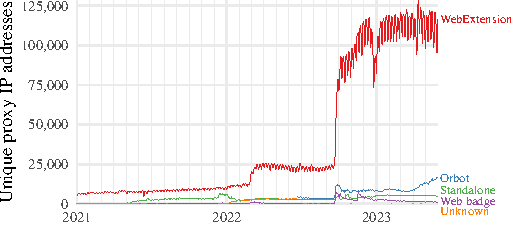
\includegraphics{figures/proxies/proxy-type}
\caption{
Unique proxy IP addresses per day,
by proxy type.
The two large steps visible in the graph correspond
to the invasion of Ukraine by Russia in late February~2022,
% 2022-02-25 https://twitter.com/torproject/status/1497276960556429324
% 2022-02-25 https://twitter.com/0xggus/status/1497224413829283877
and protests in Iran beginning late September~2022,
% 2022-09-24 https://twitter.com/torproject/status/1573670895696183303
% 2022-10-03 https://www.eff.org/deeplinks/2022/10/snowflake-makes-it-easy-anyone-fight-censorship
at which times there were campaigns
to encourage people to install the browser extension.
}
\label{fig:proxy-type}
\todo[inline]{Decide how to handle the small number of remaining ``Unknown'' proxy types.}
% 2021-02-23 https://github.com/guardianproject/orbot/releases/tag/16.4.1-BETA-2-tor.0.4.4.6
% "experimental mode to enable running as a Snowflake proxy"
% 2021-07-14 https://github.com/tladesignz/IPtProxy/commit/228e9e61e285ee548a42d6bee487577e44630695
% IPtProxy 1.1.0 changes its proxy type from "standalone" to "iptproxy"
% 2021-12-20 https://github.com/guardianproject/orbot/releases/tag/16.5.2-RC-1-tor.0.4.6.8
% Orbot updates IPtProxy from 1.0.0 to 1.2.0 https://github.com/guardianproject/orbot/commit/57add48cd904afe94363219887cd142bb5cf6696
% 2022-01-03 https://github.com/guardianproject/orbot/releases/tag/16.5.2-RC-5-tor.0.4.6.9
% This is close to the date (2022-01-05) when there's sudden growth in "Unknown",
% which is probably Orbot self-reporting as "iptproxy" and the broker throwing away that label for being unrecognized.
% 2022-03-21 https://gitlab.torproject.org/tpo/anti-censorship/pluggable-transports/snowflake/-/merge_requests/82
% Broker starts to recognize "iptproxy" as a probe type, but not deployed yet.
% 2022-05-03 https://github.com/tladesignz/IPtProxy/commit/c6ba25ef6ce8449476f734c626eadffdf55d0519
% IPtProxy 1.6.0 adds 'ProxyType: "iptproxy"' (no effective change, had already been done in a patch).
% 2022-06-21 https://bugs.torproject.org/tpo/anti-censorship/pluggable-transports/snowflake/40151
% Broker deployment, broker starts recording "iptproxy" in descriptors.
% 2022-07-05 https://github.com/guardianproject/orbot/releases/tag/16.6.2-RC-1-tor.0.4.7.8
% Orbot 16.6.2 RC 1 upgrades to IPtProxy 1.6.0.
% 2022-08-02 https://github.com/guardianproject/orbot/releases/tag/17.0.0-ALPHA-1-tor.0.4.7.8
% "updated UI based on new design spec: https://github.com/guardianproject/orbot/blob/NEW_UX/docs/design-spec-kindness-mode.md"
% "improved support for Snowflake Proxying "kindness" / volunteer mode"
% 2023-01-13 https://github.com/guardianproject/orbot/releases/tag/17.0.0-BETA-1-tor.0.4.7.11
% "easy access to Snowflake proxy 'kindness' mode"
\end{figure}

Snowflake's effectiveness depends on its proxies,
of~which there are several types.
The primary type is the web browser extension,
% "Creating a Snowflake WebExtension addon" https://bugs.torproject.org/tpo/anti-censorship/pluggable-transports/snowflake/23888
which, once installed, works in the background
while the browser is running.
There is also a ``web badge'' version of the proxy that does not require installation.
It~uses the same JavaScript code as the extension, but runs in an ordinary web page.
Some people leave a browser tab idling on the web badge page,
rather than install a browser extension.
Apart from the web-based proxies,
we~provide a standalone, command-line proxy
that does not require a browser.
% "Golang implementation of standalone snowflake proxy" https://github.com/keroserene/snowflake/pull/41
This version is convenient to install on a rented VPS, for example.
Running a long-term proxy at a fixed IP address
is somewhat at odds with Snowflake's goal of proxy address diversity and agility,
but these standalone proxies are valuable because
they tend to have less restrictive NATs,
making them compatible with more clients.
Finally, Orbot, a mobile app for accessing Tor,
besides being able to \emph{use} Snowflake for circumvention,
can also \emph{provide} Snowflake proxy service to others,
a~feature called ``kindness mode.''
% Only so called in Orbot v17+, which should be current by the time the paper is submitted.

\autoref{fig:proxy-type} shows the daily counts
of each proxy type.
Browser extension proxies predominate,
representing about 88\%\todo{Update percentage before submission.}
of 125,000 daily IP addresses.
% > read_csv("figures/proxies/proxy-type.csv", col_types = cols()) %>% filter("2023-04-01" <= date & date < "2023-04-08") %>% group_by(type) %>% summarize(unique_ips = sum(unique_ips)) %>% mutate(percent = 100 * unique_ips / sum(unique_ips)) %>% ungroup()
% # A tibble: 4 x 3
%   type       unique_ips percent
% * <chr>           <dbl>   <dbl>
% 1 badge           9506.    1.08
% 2 iptproxy       63035.    7.16
% 3 standalone     35749.    4.06
% 4 webext        772422.   87.7
For comparison, there were about 2,000
of the more traditional style of Tor bridge at this time.
% https://metrics.torproject.org/networksize.html?start=2023-05-01&end=2023-05-31
% date,relays,bridges
% 2023-05-29,6702,2126
% 2023-05-30,6712,2137
% 2023-05-31,6750,2129
The difference is attributable to the relative ease
of running a Snowflake proxy versus a Tor bridge---though
the comparison is not quite direct,
because Tor bridges have better defenses
against enumeration and blocking than do Snowflake proxies.

It~was not clear at the outset
that it would even be possible to attract
enough proxies to make Snowflake meaningfully blocking resistant
and support a reasonable number of users.
% "Start producing snowflakes" https://bugs.torproject.org/tpo/anti-censorship/pluggable-transports/snowflake/20813
Initial growth in the number of proxies
depended on our developing new and easier ways to run one,
while later growth was driven by intentional advocacy and outreach.
In~the early days, circa~2017,
the only round-the-clock proxy support was
a few standalone proxies,
% 2018 "The three fallback proxy-go instances..." https://bugs.torproject.org/tpo/anti-censorship/pluggable-transports/snowflake/25688
run by us for the benefit of alpha tester clients.
The browser extension became available in mid-2019.
% |2019-06-26|||snowflake|Deployed version 0.0.1 of the Snowflake WebExtension for Firefox.|[comment](https://bugs.torproject.org/tpo/anti-censorship/pluggable-transports/snowflake/30931#note_2593598)||
% |2019-07-03|||snowflake|Deployed version 0.0.1 of the Snowflake WebExtension for Chrome.|[comment](https://bugs.torproject.org/tpo/anti-censorship/pluggable-transports/snowflake/30999#note_2593718)||
In~the latter half of 2019,
% |2019-07-26|||flashproxy snowflake|Cupcake 2.0 is released, now working with Snowflake rather than flash proxy.|[Chrome Web Store page](https://chrome.google.com/webstore/detail/cupcake/dajjbehmbnbppjkcnpdkaniapgdppdnc)||
% Cupcake stopped working when we changed the proxy–broker protocol:
% |2019-11-13 16:47:02|||snowflake|Restarted the broker with a new proxy–broker protocol.|[comment](https://gitlab.torproject.org/tpo/anti-censorship/pluggable-transports/snowflake/-/issues/29207#note_2592849)||
additional proxy capacity came when Cupcake,
a~browser extension for flash proxy with an existing user base,
was repurposed for Snowflake.
% "Link Cupcake from snowflake.torproject.org" https://bugs.torproject.org/tpo/anti-censorship/pluggable-transports/snowflake/31497
% "Snowflake integration" https://github.com/glamrock/cupcake/issues/24
Orbot's Snowflake proxy feature was added in version 16.4.1 in February~2021.
% https://github.com/guardianproject/orbot/releases/tag/16.4.1-BETA-2-tor.0.4.4.6 2021-02-23
% https://github.com/guardianproject/orbot/releases/tag/16.4.1-RC-1-tor.0.4.4.6 2021-04-09
% https://github.com/guardianproject/orbot/blob/a69f39bb37469e65730d0751519848ec29001959/CHANGELOG#L714 /** 16.4.1-RC-1 / 9 April 2021 / c80f18ae2508b73fcbfd6e09b394a2a196de7459 **/
% https://lists.mayfirst.org/pipermail/guardian-dev/2023-July/005708.html
% 16.4.1-BETA-2-tor.0.4.4.6 was released and promoted first, and had a visible effect on proxy counts,
% though 16.4.1-RC-1-tor.0.4.4.6 was the "real" 16.4.1 release.
(In~\autoref{fig:proxy-type}, Orbot is counted among the standalone proxies
until January~2022, when it got its own proxy type designation.)
% See history in figures/proxies/proxy-type.r.

It~is worth reflecting briefly
on the greater popularity of the browser extension
compared to the web badge.
The latter had been envisioned
as the primary source of proxies in flash proxy,
% By the end of its run, flash proxy had also gained
% https://www.bamsoftware.com/talks/ee380-flashproxy/index.html#s15
% browser extensions including Cupcake
% "Chrome browser add-on" [Cupcake for flash proxy] https://bugs.torproject.org/legacy/trac/7721
% "Tor Flashproxy Badge" [for Firefox] https://github.com/reezer/tor-flashproxy-badge/
% and a standalone proxy.
% "Node.js standalone flash proxy" https://bugs.torproject.org/legacy/trac/7944
the idea being that people's browsers
would automatically become proxies
while reading sites that had the flash proxy badge installed,
unless they checked an option to prevent~it.
We~decided, early on, that flash proxy's opt-out permission had been a mistake,
% Date: Tue, 6 Dec 2016 18:38:40 -0800
% From: David Fifield <dcf@torproject.org>
% To: Arlo Breault <arlo@torproject.org>
% Cc: Serene <serene@torproject.org>
% Subject: Re: Snowing
% Message-ID: <20161207023840.mli4cymr6s3aanpu@happy.bamsoftware.com>
%
% My original plan was to repurpose existing flash proxy badges as
% Snowflake badges. But, I am thinking more and more that Snowflake should
% use an opt-in model, rather than opt-out. The opt-out model of flash
% proxy always bothered me. I think there's a good chance it would cause
% trouble for us if Snowflake becomes popular. So I'd like to see
% Snowflake use opt-in badges (and Cupcake) only.
and that Snowflake would be only opt-in.
In~order to run a proxy, a person must to take a positive action
such as installing a browser extension
or activating a toggle on a web page.
% "Prepare a Snowflake 'options' page, like in flashproxy" https://github.com/keroserene/snowflake/issues/21
Our initial worry that this policy
would reduce the number of proxies turned out to be unfounded.
People find an informative, interactive proxy control panel more appealing
than a nondescript badge graphic,
and install the browser extension in greater numbers
than ever used the web badge in flash proxy.

\subsection{Proxy churn}
\label{sec:proxy-churn}

% https://bugs.torproject.org/tpo/anti-censorship/pluggable-transports/snowflake/34075
% https://gitlab.torproject.org/tpo/anti-censorship/pluggable-transports/snowflake/-/merge_requests/95

The size of the proxy pool is not the only measure of its quality.
Also important is its ``churn,'' the rate at which
it is replenished with fresh proxy IP addresses.
Churn determines how hard a censor would have to work
to keep a blocklist of proxy IP addresses up to date;
or alternatively,
how quickly a momentarily complete blocklist
would lose effectiveness.

We ran an experiment to measure churn.
Every hour, the broker logged a record of
the proxy IP addresses it had seen in the past hour.
To~avoid storing real proxy IP addresses,
each record was not a transparent list,
but a HyperLogLog++ sketch~\cite{Heule2013a},
a~probabilistic data structure for estimating
the number of distinct elements in a multiset.
We~additionally hashed proxy IP addresses with a secret string
before adding them to a sketch,
to prevent their recovery from our published data.
A~sketch supports two basic operations: count and merge.
Given a sketch~\(X\),
we may compute an approximate count \(|X|\)
of its unique elements,
and given two sketches \(X\) and~\(Y\),
we~may merge them into a new sketch
representing the union \(X \cup Y\).
The quantity we are interested in,
the size of the intersection of two sketches,
is~computed using the formula
\(|X| + |Y| - |X \cup Y|\).
Such a computation estimates
how many IP addresses are shared across
two samples of the proxy pool.

\begin{figure}
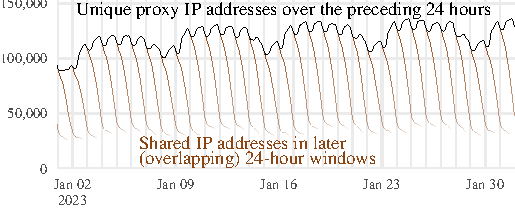
\includegraphics{figures/proxy-churn/proxy-count-decay}
\caption{
Proxy pool churn in January 2023.
The dark upper line shows the number
of unique proxy IP addresses in a 24-hour window
starting at the point indicated.
The lighter descending lines show
how many of the same IP addresses remain in the pool,
at 1-hour intervals up to 40 hours later.
It~takes about 20~hours for 50\% of the proxy pool to turn over.
}
\label{fig:proxy-count-decay}
\end{figure}

\autoref{fig:proxy-count-decay}
visualizes the results of the churn experiment.
We merged consecutive sketches over a 24-hour window
to serve as a reference,
then computed the size of its intersection
with other windows of the same size,
offset by \(+1, +2, \ldots, +40\) hours.
After 1~hour, the shifted window still has, on average,
97.3\% of addresses in common with the reference;
after 12~hours the fraction has fallen to 68.8\%;
by the time 24~hours have elapsed,
only 38.2\% of proxy IP addresses
are ones that had been seen in the previous day.
% > library("tidyverse")
% > options(width = 200)
% > DATE_RANGE <- as.Date(c("2023-01-01", "2023-02-01"))
% > read_csv("figures/proxy-churn/proxy-churn-windows.csv") %>%
%     filter(lubridate::`%within%`(reference_timestamp_end, do.call(lubridate::interval, as.list(DATE_RANGE)))) %>%
%     mutate(
%       sample_offset_hours = round(sample_timestamp_end_offset / 3600),
%       intersection_count = reference_count + sample_count - union_count
%     ) %>%
%     group_by(sample_offset_hours) %>%
%     summarize(
%       across(c(reference_count, sample_count, union_count, intersection_count), mean),
%       intersection_percent = 100 * intersection_count / reference_count,
%       .groups = "drop"
%     ) %>%
%     filter(sample_offset_hours %in% c(0, 1, 2, 3, 4, 8, 12, 18, 24, 36, 40))
% # A tibble: 11 x 6
%    sample_offset_hours reference_count sample_count union_count intersection_count intersection_percent
%                  <dbl>           <dbl>        <dbl>       <dbl>              <dbl>                <dbl>
%  1                   0         119654.      119654.     119654.            119654.                100
%  2                   1         119654.      119704.     122907.            116450.                 97.3
%  3                   2         119654.      119754.     126142.            113266.                 94.7
%  4                   3         119654.      119804.     129359.            110099.                 92.0
%  5                   4         119654.      119854.     132529.            106980.                 89.4
%  6                   8         119654.      120060.     145141.             94572.                 79.0
%  7                  12         119654.      120292.     157684.             82262.                 68.8
%  8                  18         119654.      120649.     176400.             63903.                 53.4
%  9                  24         119654.      120970.     194892.             45732.                 38.2
% 10                  36         119654.      121500.     206542.             34612.                 28.9
% 11                  40         119654.      121639.     208269.             33024.                 27.6

\subsection{Multiple bridges}
\label{sec:multi-bridge}

% "Prepare all pieces of the snowflake pipeline for a second snowflake bridge" https://bugs.torproject.org/tpo/anti-censorship/pluggable-transports/snowflake/28651
% "Distributed Snowflake Server Support" https://bugs.torproject.org/tpo/anti-censorship/pluggable-transports/snowflake/40129
% Ancient history from flash proxy: "allow the client to pick a specific relay for its registration" https://bugs.torproject.org/legacy/trac/10196

The bridge in the Snowflake model (\autoref{sec:mechanics})
is notionally a single, centralized entity.
It~\emph{can} be centralized
because it is insulated from direct blocking
by the snowflake proxies.
Unlike traditional proxy systems,
Snowflake does not benefit, in terms of blocking resistance,
by having multiple bridges,
since the bridge is decoupled from the means of accessing it.
For practical performance reasons, though,
it makes sense for ``the'' bridge to be realized as
multiple servers, simply because the load of Snowflake traffic
is a lot for one server to handle.
\todo{Note fraction of total Tor traffic.}
For technical reasons, though,
the use of multiple bridges cannot be made fully transparent to clients
without making some compromises.
One of the reasons, relatively minor, is related to Snowflake itself;
the other, more constraining one has to do with its interaction with Tor.
We will explain the tradeoffs involved
and the design we settled on.

What is called the bridge is actually a pipeline of several components.
One component terminates incoming WebSocket connections arriving from proxies,
one decodes the Turbo Tunnel packets contained therein and reassembles them into streams,
and one forwards the streams to their eventual destinations
(in~our deployment, this last component is Tor itself).
These components are separable.
For example, because the interface with Tor is ordinary TCP sockets,
it is easy to run Tor on a different host with its own CPU and RAM,
% A diagram of such separation: https://bugs.torproject.org/tpo/anti-censorship/pluggable-transports/snowflake/28651#note_2783541
or even round-robin over multiple instances of Tor
(as we in fact do~\cite{Fifield2023a}).

What is not so easy to distribute
is the Turbo Tunnel layer itself.
Recall from \autoref{sec:data-transfer} that Snowflake
has a notion of a long-term end-to-end session
between the client and the bridge that is independent of
the temporary proxies in between.
This is made possible by extensive state stored at the bridge:
a table of ongoing sessions, reassembly buffers,
transmission queues, timers, and so on.
% `type KCP` https://github.com/xtaci/kcp-go/blob/03b584b84eddd95cc03dbff65fc9cc5cbdf80c6b/kcp.go#L132
% `type UDPSession` https://github.com/xtaci/kcp-go/blob/03b584b84eddd95cc03dbff65fc9cc5cbdf80c6b/sess.go#L61
While it is certainly possible to instantiate more than one such state machine,
a~session that is begun in one instance must remain in that instance---any
other instance will not have the state necessary to make the packets
of the session meaningful.

The other difficulty is a Tor bridge is identified
by a \firstterm{bridge fingerprint},
a hash of its long-term Tor identity key.
The bridge configuration interface in the Tor client
expects a bridge fingerprint,
and if the bridge it connects to cannot prove that
its identity matches that fingerprint,
the client will terminate the connection~\cite[\S 5.1.2]{tor-spec}\todo{Verify that this is the relevant section of the spec.}.
% https://gitweb.torproject.org/torspec.git/tree/tor-spec.txt?id=33308845cec54bfc0096b8ea0339a8ff183aa1b1#n1153
% "Extending ORs MUST check _all_ provided identity keys (if they recognize the format), and and MUST NOT extend the circuit if the target OR did not prove its ownership of any such identity key."
There is no facility in Tor for a certificate,
or anything like that,
to authorize a whole set of equivalent bridge fingerprints:
the fingerprint of every bridge a client may use
must be configured separately at the client.
While it is possible to copy identity keys between
separate instances of Tor so they have the same fingerprint,
and desirable to do so within one bridge installation for performance reasons,
our vision for scaling the Snowflake backend
involved bridge sites in different locations,
managed by different teams,
and we decided that we did not want the trust boundary
of who has access to those important keys to be quite so large.

In short, the client must know in advance which bridge
its snowflake proxy will connect (or re-connect) it to.
If~the first connection is to a bridge other than the one the client expects,
the Tor client will abandon the connection because the bridge fingerprint is wrong.
Subsequent re-connections in the same client session
need to go to the same bridge,
otherwise the Turbo Tunnel session state will be missing.

These considerations led us to a multi-bridge design
in which the client has awareness of (at least a subset of)
all the bridges that exist,
and it is the client that chooses which bridge will be used
for a particular session.
The client includes a bridge fingerprint
in its rendezvous message (\autoref{sec:rendezvous}) to the broker;
the broker maps the fingerprint to a WebSocket URL,
and conveys that URL to the proxy.
We~rely on clients choosing uniformly
to equalize the load across bridges.
A~consequence is that
every bridge must meet some minimum performance standard:
we cannot, say,
assign 20\% of clients to one and 80\% to another
according to their relative capabilities.
A~further drawback is that there is no way to try connecting
to only one of the bridges it knows about,
short of rewriting the configuration file;
if two bridges are configured, Tor will start two sessions through Snowflake,
each doing its own independent rendezvous,
which is wasteful and makes the network fingerprint more conspicuous.
% "Let bridge users choose to only reach their first working bridge" https://bugs.torproject.org/tpo/core/tor/40578
Still, this is the best solution we have found, given the limitations.
A~deployment not based on Tor would have more flexibility here.
The only consideration would be the Turbo Tunnel session state,
which could be solved by hashing a client's session identifier string
to consistently assign the same bridge during a session.

A~client-chooses design risks the possibility
of misuse by clients, if not handled carefully.
The client should be able to select
a proxy destination from the set of known bridges,
but not cause a proxy to connect to arbitrary destinations,
otherwise the many proxies of \autoref{sec:proxies}
could be used to attack third parties.
% "Clients cannot cause a proxy to attack or even connect to an arbitrary web site or relay..." https://forum.torproject.net/t/anyone-experiencing-problems-with-snowflake-proxy/6938/15
% An alternative vision: "(More) Distributed servers" https://bugs.torproject.org/tpo/anti-censorship/pluggable-transports/snowflake/40248
When the client expresses its bridge selection
in its rendezvous message, the selection is represented
not as an IP address or hostname,
but as a bridge fingerprint (a~\mbox{40-digit} hexadecimal string).
The broker maps the fingerprint to a WebSocket URL
by consulting a local database of known Snowflake bridges.
The broker rejects client rendezvous messages requesting an unknown fingerprint.
% https://gitlab.torproject.org/tpo/anti-censorship/pluggable-transports/snowflake/-/blob/8e5ea8261110e97a8df56cfc9c83028081d902fb/broker/ipc.go#L187
The broker then tells an incoming proxy
what WebSocket URL to connect this particular client to,
% https://gitlab.torproject.org/tpo/anti-censorship/pluggable-transports/snowflake/-/blob/8e5ea8261110e97a8df56cfc9c83028081d902fb/broker/ipc.go#L144
but here also there is a check.
Proxies check the hostname of the URLs
to ensure that it is a subdomain of a known suffix reserved for Snowflake bridges.
So~there are two independent safeguards against misuse.

As~of May 2023\todo{Update on publication.},
there are two Snowflake bridges,
which are among the largest relays in the Tor network,
in terms of bandwidth.\todo{Do some analysis from figures/\allowbreak onionoo.}
% Actually head-and-shoulders the largest relays?
% figures/onionoo$ jq -r '(.relays+.bridges)|sort_by(-.advertised_bandwidth)[]|[.nickname,.advertised_bandwidth]|@tsv' top-consensus_weight.onionoo.json | head -n 4
% RandomRecipes	114341160
% poiuty	109014582
% xor	103805661
% StayStrongRelay01	99326969
% figures/onionoo$ jq -r '(.relays+.bridges)|sort_by(-.advertised_bandwidth)[]|[.nickname,.advertised_bandwidth*12]|@tsv' snowflake-??.onionoo.json
% flakey6	467165892
% crusty7	178083996

% https://archive.is/aYyxR 2023-04-29 archive of https://metrics.torproject.org/rs.html#toprelays
% https://archive.is/zOp4G 2023-04-29 archive of https://metrics.torproject.org/rs.html#aggregate/as
% https://archive.is/GHBKE 2023-04-29 archive of https://metrics.torproject.org/rs.html#details/5481936581E23D2D178105D44DB6915AB06BFB7F (snowflake-01) (multiply by 12)
% https://archive.is/LKFxo 2023-04-29 archive of https://metrics.torproject.org/rs.html#details/91DA221A149007D0FD9E5515F5786C3DD07E4BB0 (snowflake-02) (multiply by 12)
% Relay bandwidth aggregated by AS: https://metrics.torproject.org/rs.html#aggregate/as; on 2023-04-29 Snowflake bridges provide about as much advertised bandwidth as Emerald Onion.

% \subsection{SQL injection attempts at broker}
% \url{https://bugs.torproject.org/tpo/anti-censorship/pluggable-transports/snowflake/40089}
% Actually tailored to the broker protocol, not a generic attack tool.

\section{Notable blocking attempts}
\label{sec:block}

We have seen Snowflake's user counts in \autoref{sec:deployment},
and remarked on how they have at times been affected by blocking actions by censors.
Now we take a closer look at the technical details of specific censorship events.
The effect of these has usually been to increase rather than decrease
the number of Snowflake users.
Though seemingly paradoxical, this effect is easy to explain:
as the intensity of censorship increases,
users are displaced from less resilient systems
to more resilient systems.
Snowflake's blocking resistance has not in every case been an unqualified success,
though, and here we also reflect on missteps
and persistent challenges.

The examples are taken from
Russia, Iran, and Turkmenistan,
and are selected for being significant and instructive.
Only in Russia was the blocking action clearly targeted at Snowflake specifically;
in~the other cases the blocking rules were broad enough
that they may have affected Snowflake only indirectly.
Common themes are that having a line of communication
with affected users is invaluable in understanding and reacting to blocking;
and that a circumvention system's blocking resistance
can only be understood in relation to a censor,
because every censor's cost calculus is different.

Snowflake is blockable by any censor that is willing to block all WebRTC.
We~would not try to claim otherwise.
Indeed, we believe that is the way circumvention systems
should be presented:
not to argue their unblockability in universal terms,
but by specifying, as completely as possible,
what actions by the censor would suffice to block it---or
more to the point,
\emph{what sacrifices a censor would have to make}
in order to block~it.
Some censors may be able to make those sacrifices; others may not.
Advancing the state of the art in censorship circumvention
consists of finding techniques that put blocking
farther out of reach of would-be controllers of information.
\todo{Reflect on a good location to place this sentiment.}

\begin{figure}[t!]
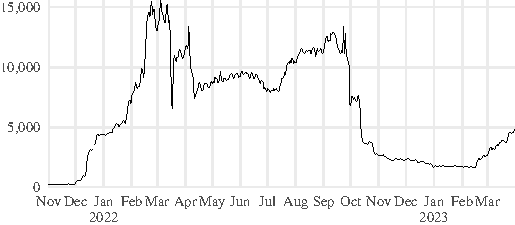
\includegraphics{figures/users/users-ru}
\caption{
Snowflake users in Russia (average concurrent).
The blocking of Tor-related transports in December~2021
led to Snowflake's first surge in usage.
The decrease in September~2022
coincided with an even larger influx of users from Iran,
which may have masked another blocking rule.
}
\label{fig:user-counts-ru}
\bigskip
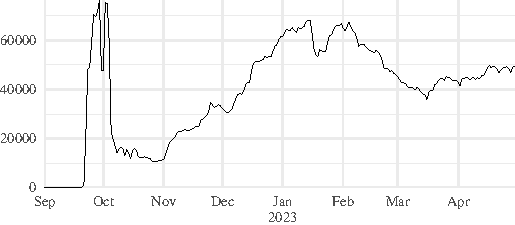
\includegraphics{figures/users/users-ir}
\caption{
Snowflake users in Iran.
The censorship that followed
protests that started in September 2022
caused Iran to suddenly become the largest contingent of Snowflake users.
The drop in early October 2022
was the result of blocking based on TLS fingerprint,
which interfered with Snowflake's rendezvous
and took some time to mitigate.
}
\label{fig:user-counts-ir}
\bigskip
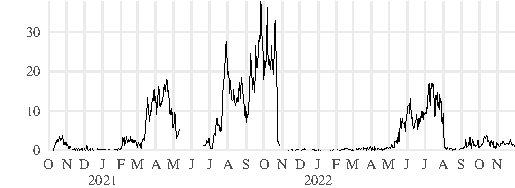
\includegraphics{figures/users/users-tm}
\caption{
Snowflake users in Turkmenistan.
Though there have never been many Snowflake users in Turkmenistan,
blocking actions are evident on
\mbox{2021-10-24} and \mbox{2022-07-28}.
}
\label{fig:user-counts-tm}
\todo[inline]{Add annotations for specific events, like in \autoref{fig:user-counts}.}
\end{figure}

\subsection{Blocking in Russia}
\label{sec:block-ru}

% "[Russia] Some ISPs are blocking Tor" https://bugs.torproject.org/tpo/community/support/40050
% "OONI reports of Tor blocking in certain ISPs since 2021-12-01" https://ntc.party/t/ooni-reports-of-tor-blocking-in-certain-isps-since-2021-12-01/1477
% "Responding to Tor censorship in Russia" https://blog.torproject.org/tor-censorship-in-russia/

Snowflake, along with other common ways of accessing Tor,
was blocked in a subset of ISPs in Russia
% https://ntc.party/t/ooni-reports-of-tor-blocking-in-certain-isps-since-2021-12-01/1477/95
% "Tor filtering is done using government black box called TSPU.
% Not all providers have them. Tor is not blocked if TSPU is not present.
% According to tor metrics graph directly connecting users decreased only by 1/3.
% This indicates TSPU is not everywhere."
\todo{Consider introducing TSPU? Or not?}
on \mbox{2021-12-01}~\cite{ooni-2021-russia-blocks-tor}.
The blocking action was clearly pre-planned and targeted,
as it happened suddenly and affected multiple Tor-related protocols.
Besides Snowflake,
the IP addresses of a portion
of unobfuscated Tor relays and bridges,
as well as some servers of
the blocking-resistant transports meek and obfs4,
were blocked, at least temporarily.
As~you might expect, the attempt to block
various blocking-resilient transports
was less than totally successful,
and the ultimate effect was a substantial increase in the number
of users accessing Tor via circumvention transports,
Snowflake among them---see the left side of \autoref{fig:user-counts-ru}.
% "A zoom on just the bridge transports" https://bugs.torproject.org/tpo/community/support/40050#note_2796770
% That pluggable transports could not compensate fully
% for the loss of relay users points to a usability gap.
For an overview of how Tor-related transports were affected at this time,
see an article by Ramesh, Sundara Raman, et~al.~\cite[\S 6.2]{Ramesh2023a}.
Here, our focus is on Snowflake.

We~had the benefit of established relationships
and communication with developers and users in Russia,
one of whom, through manual tests, was able to
isolate the traffic feature used to distinguish Snowflake.
It~was DTLS fingerprinting,
of the kind cautioned about in \autoref{sec:fingerprinting}.
% "Russian DPI check supported_groups extension in ServerHello payload (byte 0x5a in udp packet)." https://bugs.torproject.org/tpo/anti-censorship/pluggable-transports/snowflake/40014#note_2765074
Specifically, it was the presence of a
\mbox{supported\_groups} extension in the DTLS Server Hello message produced by Pion.
The extension's presence in Server Hello was actually a bug,
% "Server Hello should not contain supported_groups extension (extension.SupportedEllipticCurves)" https://github.com/pion/dtls/issues/409
but technical details of the distinguisher do not matter
so much as the practical effect,
which was that it provided the censor a byte pattern to match on
that would detect DTLS connections with a Pion implementation in the server role,
without affecting other forms of WebRTC.
The process of identifying the flaw, fixing it,
and shipping new releases of Tor Browser took two or three weeks,
% "Point to a forked version of pion/dtls with fingerprinting fix" https://gitlab.torproject.org/tpo/applications/tor-browser-build/-/merge_requests/375
% 2021-12-14 https://blog.torproject.org/new-release-tor-browser-115a1/
% 2021-12-20 https://blog.torproject.org/new-release-tor-browser-1103/
after which the user count rose quickly:
between the beginning to the end of December~2021,
the number of users in Russia grew from about 400 to about 4,000.
% > library("tidyverse")
% > WANTED_FINGERPRINTS <- c(
%     "7659DA0F96B156C322FBFF3ACCC9B9DC01C27C73" = "snowman",
%     "5481936581E23D2D178105D44DB6915AB06BFB7F" = "snowflake-01",
%     "91DA221A149007D0FD9E5515F5786C3DD07E4BB0" = "snowflake-02"
%   )
% > userstats <- read_csv("figures/users/userstats-bridge-combined-multi.csv") %>%
%     filter(transport == "snowflake" & fingerprint %in% names(WANTED_FINGERPRINTS)) %>%
%     mutate(across(c(low, high), ~ .x / (coverage / pmax(num_instances, coverage)))) %>%
%     mutate(users = (low + high) / 2) %>%
%     # Combine the contributions of all bridges.
%     group_by(date, transport, country) %>% summarize(across(c(low, high, users), sum), .groups = "drop") %>%
%     # Apportion "??" to other countries (see figures/users/users-country.r).
%     group_by(date, transport) %>% mutate(across(c(low, high, users), ~ .x * sum(.x) / sum(ifelse(country == "??", 0, .x)))) %>% ungroup() %>% filter(country != "??")
% > userstats %>% filter(date %in% as.Date(c("2021-12-01", "2022-01-01"))) %>% filter(country == "ru")
% # A tibble: 2 x 6
%   date       transport country   low  high users
%   <date>     <chr>     <chr>   <dbl> <dbl> <dbl>
% 1 2021-12-01 snowflake ru       381.  381.  381.
% 2 2022-01-01 snowflake ru      4381. 4380. 4380.
Snowflake was to become a significant tool
amid the general intensification of censorship in Russia
following the invasion of Ukraine in February~2022.

The \mbox{supported\_groups} in Server Hello distinguisher had already been
discovered and documented by MacMillan et~al.~\cite[\S 3]{arxiv.2008.03254} in~2020.
We~might have avoided this blocking event by proactively fixing
the known distinguisher,
but it was not necessarily the wrong call not to have done~so.
In~a software project like Snowflake,
there is always more to do than time to do it;
work on one task comes at the expense of some other,
possibly even more important task.
In~this case, a reactive approach by us was enough.
We~add that not only did the Snowflake block affect
only a fraction of ISPs in Russia,
it was not effective at blocking all Snowflake DTLS connections
even in the ISPs in which it was present.
If~the DTLS server role in the WebRTC data channel
was played by a web browser proxy, which is common,
then the specific Server Hello feature used by the censor
would not be present.
% The Snowflake client would retry its rendezvous repeatedly,
% until hitting on a proxy that worked.

% "IRC Tip about Signature used to block Snowflake in Russia, 2022-May-16" https://bugs.torproject.org/tpo/anti-censorship/censorship-analysis/40030
% "Snowflake blocked by ClientHello [RU]" https://bugs.torproject.org/tpo/anti-censorship/pluggable-transports/snowflake/40140
% "A new Snowflake blocking rule (offset of supported_groups in DTLS Client Hello)" https://ntc.party/t/a-new-snowflake-blocking-rule-offset-of-supported-groups-in-dtls-client-hello/2420

In~May 2022 we got a report of a new detection rule,
this time keyed on not just the presence, but the \emph{contents}
of the \mbox{supported\_groups} extension,
at a byte offset suggesting that this time
it targeted the Client Hello message,
not Server Hello.
The presence of \mbox{supported\_groups} in Client Hello is not at all unexpected,
but the specific groups offered by Pion's implementation
differed from those of common browsers.
Despite confirming the new blocking rule,
testers reported that Snowflake continued to work---which
% https://bugs.torproject.org/tpo/anti-censorship/censorship-analysis/40030#note_2804998
% https://ntc.party/t/a-new-snowflake-blocking-rule-offset-of-supported-groups-in-dtls-client-hello/2420/2
may have something to do with the fact that the Snowflake client
does not always play the client role in DTLS:
if~the Snowflake client is the DTLS server,
and the DTLS client is a browser proxy,
then the specific byte pattern of the blocking rule never appears.
% Hard to say at this point, but perhaps it was the cause of the sharp drop in April 2022, only reported in May?
Nevertheless, we developed a mitigation,
but by the time we had prepared a testing release,
% "Creating a version of Tor Browser with patched Snowflake client that includes supported_groups censorship countermeasure" https://bugs.torproject.org/tpo/anti-censorship/team/83
% https://ntc.party/t/testing-invitation-for-tor-browser-with-supported-groups-patch-countermeasure-in-snowflake-to-evade-censorship-observed-in-russia/2837
the \mbox{supported\_groups} in Client Hello rule
had apparently been removed
and replaced by another.
We~can only speculate as to motivations,
but it may be that the censor decided the old rule
had too many false positives,
or was simply not effective enough.

% "Блокировку Сlient Hello убрали, теперь блокируют Hello Verify Request" https://ntc.party/t/in-case-snowflake-rendezvous-gets-blocked/1857/9
% "They removed the blocking of Client Hello, now they block Hello Verify Request" https://bugs.torproject.org/tpo/anti-censorship/censorship-analysis/40030#note_2823140

The detection rule that replaced \mbox{supported\_groups} in Client Hello
looked for the presence of a DTLS Hello Verify Request message.
Hello Verify Request is an anti-denial-of-service measure,
in which the server sends a random cookie to the client,
and the client repeats its Client Hello message,
echoing the cookie~\cite[\S 5.1]{rfc9147}.
The presence of Hello Verify Request is not an error
(it is a ``MAY'' in the RFC),
but because the Pion implementation used by Snowflake sent it,
and major browsers did not,
it was a reliable indicator of Snowflake connections.
(Those, at least, in which the DTLS server role was played by a Pion implementation,
whether a Snowflake client or standalone proxy.)
The Hello Verify Request distinguisher had also been anticipated by
MacMillan et~al.~\cite[\S 3]{arxiv.2008.03254}.
The first reports of this blocking rule appeared in July~2022;
as you can see from \autoref{fig:user-counts-ru},
it had no apparent immediate effect.
It~is hard to say whether the drastic decline in October 2022
was a consequence of this rule,
or some other, unidentified one:
that was the same time as an explosion of users from Iran,
which temporarily affected the system's usability.
We deployed a mitigation to remove the Hello Verify Request message
from Snowflake DTLS, regrettably, only in February~2023, % and only in Tor Browser, no Orbot yet
after which the number of users began to recover.
% "Apply Snowflake Remove HelloVerify Countermeasure" https://gitlab.torproject.org/tpo/applications/tor-browser-build/-/merge_requests/637
% "Since the release of Tor Browser 12.0.3 on 2023-02-15 there has been an increase in users from Russia on both bridges." https://bugs.torproject.org/tpo/anti-censorship/censorship-analysis/40030#note_2893870

The example of Snowflake in Russia
illustrates the difficulty of censorship measurement.
The~answer to the question ``Does Snowflake work in Russia?''
is not a simple yes or~no.
It~may depend on the date, the ISP,
and even such factors as which endpoint plays the DTLS server role.

\subsection{Blocking in Iran}
\label{sec:block-ir}

% "Unexplained drop in Snowflake client polls and bandwidth, testers wanted" https://github.com/net4people/bbs/issues/131
% "Tor censorship in Iran" https://bugs.torproject.org/tpo/anti-censorship/team/96#note_2840481
% "Sudden reduction in snowflake-01 bridge bandwidth, 2022-10-04 17:15" https://bugs.torproject.org/tpo/anti-censorship/pluggable-transports/snowflake/40207
% "Planning response to censorship in Iran with AC team" https://gitlab.torproject.org/tpo/team/-/wikis/Planning-response-to-censorship-in-Iran-with-AC-team

We have remarked in \autoref{sec:deployment} how,
in late September 2022,
almost overnight Iran became the source of the majority of Snowflake users,
and had an even more sudden drop two weeks later.
The cause of the drop was blocking based on TLS fingerprint,
though it took some time to diagnose this fact.
Specifically, it was a block of one of the TLS fingerprints
produced by the crypto/tls package in the standard library of
the Go programming language.

We~say ``one of'' the crypto/tls fingerprints
because there are several the package may output.
The fingerprint changed between Go~1.17 and Go~1.18
as the latter dropped default support for TLS~1.0 and~1.1
in the Client Hello message.
% https://go.dev/doc/go1.18#tls10
% supported_versions: https://www.rfc-editor.org/rfc/rfc8446#section-4.2.1
Furthermore, the TLS client reorders its offered ciphersuites
according to hardware capabilities:
if the platform has hardware-accelerated AES,
it prioritizes AES ciphersuites;
otherwise it prioritizes ChaCha ones.
The combination of these two variables
(Go~1.17 or~1.18; AES acceleration or not)
result in four distinct TLS fingerprints;
of these, only one was blocked, namely the one from
the older version of Go, without AES acceleration.
% "This all gives us a good hypothesis... It includes the fingerprints of go1.17+ crypto/tls without AES acceleration" https://github.com/net4people/bbs/issues/139#issuecomment-1280243079
% "...in native Go crypto/tls fingerprints since go1.17 is that the order of ciphersuites depends on whether the platform has support for accelerated AES-GCM" https://bugs.torproject.org/tpo/anti-censorship/pluggable-transports/snowflake/40207#note_2844163
% "When I tested the desktop version, I did it in a VM that did not emulate support for accelerated AES-GCM..." https://github.com/net4people/bbs/issues/131#issuecomment-1280284051
% "There is strong evidence of an attempt to block the native Go crypto/tls fingerprint, but not all native fingerprints produced by Go programs are blocked." https://github.com/net4people/bbs/issues/125#issuecomment-1284602875
As~it happens, only Orbot was affected
(which is more used than Tor Browser, in Iran).
At the time, Orbot was compiling the Snowflake client with Go~1.17
and Tor Browser was using Go~1.18\todo{Fix this: \href{https://bugs.torproject.org/tpo/anti-censorship/pluggable-transports/snowflake/40207\#note_2845632}{Tor Browser also used Go~1.17.}};
the mobile platforms on which Orbot runs are also less likely to
have hardware-accelerated AES
than the desktop platforms that run Tor Browser.
We~were hampered in our investigation by the fact that
OONI Probe\todo{Say what OONI is. Or, cut this detail.} used Go~1.18 to compile Snowflake,
so its measurements showed everything as normal,
even as we saw the bandwidth drop at the bridge.

That TLS fingerprinting worked to block Snowflake
was an oversight on our part.
We had in fact already implemented TLS camouflage using uTLS,
but had failed to turn it on by default.
% "uTLS for broker negotiation" https://bugs.torproject.org/tpo/anti-censorship/pluggable-transports/snowflake/40054
Activating it took only a small configuration change,
% "Enable uTLS and use the full bridge line for snowflake" https://gitlab.torproject.org/tpo/applications/tor-browser-build/-/merge_requests/540
but we had to wait out the release cycles of Tor Browser and Orbot
to get it in the hands of users:
see the September--November~2022 interval in \autoref{fig:user-counts-ir}.

The fact that only one of Snowflake's possible TLS fingerprints was blocked
(albeit the most common one)
could show carelessness on the part of the censor.
On~the other hand, it is not certain that the TLS fingerprint blocking of October 2022
was targeted specifically at Snowflake.
Go~is a popular language for implementing circumvention systems.
Snowflake may have been caught up in blocking that was intended for another system.

% "Blocking of cdn.sstatic.net by SNI in Iran, 2023-01-16 to 2023-01-24 and sporadically thereafter" https://bugs.torproject.org/tpo/anti-censorship/team/115#note_2873040

The default front domain of domain fronting rendezvous
was blocked in some ISPs, matching on the TLS SNI field,
between \mbox{2023-01-16} and \mbox{2023-01-24}.
We~confirmed this by examining OONI measurements;
there was also a reduction in users at this time (\autoref{fig:user-counts-ir}).
AMP cache rendezvous was a successful workaround while the block was in effect.
After the block was lifted,
OONI measurements in the following weeks showed isolated cases
of failure to connect to the front domain,
which may have been more blocking,
though with less intensity and not for more than a few days at a time.

\todo{Add a section for China.}
% "Hello, in China, currently, Tor Browser 8.5a11 version can't connect to Tor network through Snowflake bridge." https://bugs.torproject.org/tpo/anti-censorship/pluggable-transports/snowflake/30350
% "Hello, currently, in China, Tor Browser 9.5a2 still can't connect to Tor network through snowflake bridge" https://bugs.torproject.org/tpo/anti-censorship/pluggable-transports/snowflake/32597
%
% "Run some tests to check reachability of snowflake proxies" https://bugs.torproject.org/tpo/anti-censorship/pluggable-transports/snowflake/30368
%
% "Confirmed block of default Snowflake in China" https://github.com/net4people/bbs/issues/249
% "Snowflake bridge does not work in China since days ago" https://forum.torproject.net/t/snowflake-bridge-does-not-work-in-china-since-days-ago/7635
% "Blocking of Snowflake in China, 2023-05-12" https://bugs.torproject.org/tpo/anti-censorship/censorship-analysis/40038
%
% "Potential TLS-over-DTLS blocking in China" https://github.com/net4people/bbs/issues/255
% "Analysis of speed deficiency of Snowflake in China, 2023 Q1" https://bugs.torproject.org/tpo/anti-censorship/pluggable-transports/snowflake/40251#note_2906723
% Also note contemporaneous
% "GFW at the Edge: Latest Development of China's Distributed Censorship System" https://github.com/net4people/bbs/issues/248

\subsection{Blocking in Turkmenistan}
\label{sec:block-tm}

% "Blocking of Snowflake in Turkmenistan, 2021-10-24" https://bugs.torproject.org/tpo/anti-censorship/censorship-analysis/40024
% "On 2021-10-24, Snowflake users dropped drastically and thereafter went to zero." https://bugs.torproject.org/tpo/anti-censorship/censorship-analysis/40029#note_2787789

\todo{
Read \href{https://dl.acm.org/doi/fullHtml/10.1145/3543507.3583189}{``Measuring and Evading Turkmenistan's Internet Censorship''}
to see if it can inform this section.
}

Compared to Russia and Iran,
there had not been many Snowflake users in Turkmenistan,
likely a consequence of the lesser development
of the country's Internet infrastructure
and its even more extreme network censorship.
Nevertheless, there were some,
but on \mbox{2021-10-24} the number dropped suddenly to zero,
as~you can see in \autoref{fig:user-counts-tm}.
Our investigation found the blocking to consist of two layers:
the default domain fronting rendezvous domain was blocked
by DNS injection;
and certain UDP port numbers commonly used by STUN were blocked.
We~were able to mitigate the blocking
by providing alternative domain fronts for rendezvous
and finding public STUN servers running on non-standard ports,
but not for all users in all ISPs.
Turkmenistan remains a difficult environment for circumvention.
% had been about 750 relay users at the time
% relays dropped as well on 2021-10-29 https://bugs.torproject.org/tpo/anti-censorship/censorship-analysis/40029#note_2787789

Among the mechanisms used for censorship in Turkmenistan
are DNS injection and TCP RST injection.
DNS queries for blocked hostnames receive an injected response
containing the localhost IP address 127.0.0.1;
TLS handshakes with a blocked SNI receive an injected TCP RST packet
that terminates the connection.
% "I did some tests to see if it would be possible to measure blocking of SNI and DNS from outside Turkmenistan" https://gitlab.torproject.org/tpo/community/support/40030#note_2748011
% "Bidirectional DNS, HTTPS, HTTP injection in Turkmenistan" https://github.com/net4people/bbs/issues/80
Conveniently for analysis,
both forms of injection are bidirectional:
packets that \emph{enter} the country are subject to injection,
just as those that exit it are.
We~took advantage of this fact,
sending probes into the country,
to find that the default front domain used to access the broker
was blocked by both DNS injection and RST injection,
% "...the block on Snowflake is effected by (at least) DNS and SNI blocking of the broker's front domain, cdn.sstatic.net." https://bugs.torproject.org/tpo/anti-censorship/censorship-analysis/40024#note_2767094
but that some alternative domains were not blocked.
Testers in Turkmenistan confirmed that using a different front domain
worked to get around the block of the broker.
(We~did not get confirmation whether AMP cache rendezvous also worked.)
% "...there's some progress in the sense that the broker connection is working now, but it looks like the client is having trouble connecting to the proxies." https://bugs.torproject.org/tpo/anti-censorship/censorship-analysis/40024#note_2829140
But Snowflake still did not work,
because even after contacting the broker,
clients were not able to make a connection with a proxy.
% "connection failed timeout waiting for DataChannel.OnOpen" https://bugs.torproject.org/tpo/anti-censorship/censorship-analysis/40024#note_2829121

More rounds of testing revealed a block of the default port number
used by STUN, UDP port~3478.
% "And port 3478 is blocked in TM" https://bugs.torproject.org/tpo/anti-censorship/censorship-analysis/40024#note_2829127
Not being able to reach a STUN server,
a~client cannot find its own ICE candidate addresses
(refer to \autoref{sec:ice}),
causing the overwhelming majority of peer-to-peer connections with proxies to fail.
Although clients without STUN candidates could theoretically connect
to proxies without any NAT or firewall, most VPS providers are blocked
wholesale in Turkmenistan, leaving proxies located on residential networks
as the only option.
As~luck would have it, the NAT discovery feature we rely on
for testing the NAT type of clients also requires
STUN servers to listen on a second port other than the default~\cite[\S 6]{rfc5780}
(commonly 3479),
and changing the STUN server addresses to those other port numbers
let some users connect to Snowflake again.
% "this line... :3479... Works!" https://gitlab.torproject.org/tpo/anti-censorship/censorship-analysis/-/issues/40024#note_2829157
Specifically, STUN servers on port 3479 worked in AGTS,
one of two major affected ISPs.
\todo{Check if we can determine through our metrics how long the port 3479 bridge line worked in AGTS.}
Port~3479 was blocked in Turkmentelecom, the other major ISP,
and the workaround did not work there.
% "So the line where we switch to port 3479 only works for some people but not others?" https://bugs.torproject.org/tpo/anti-censorship/censorship-analysis/40024#note_2829235

\todo{Investigate and discuss further blocking on \mbox{2022-07-28}.}

The blocking actions just described are unsophisticated,
surely resulting in significant overblocking---but
nevertheless they offer greater challenges to circumvention
than the more considered blocking observed in Russia and Iran.
We~highlight this to make the point that the blocking resistance
of a circumvention system cannot be understood in absolute terms,
but only relative to a particular censor.
Censors differ not only in their technical capabilities
(time, money, equipment, personnel),
but also in their tolerance for the social and economic harms caused by overblocking.
Different censors value the various aspects of network access differently,
and circumvention can only respond to and act within those constraints.
The government of Turkmenistan has evidently chosen
a point on the spectrum that prioritizes political control
over a functioning network, to an extreme degree.\todo{Check that this washes with someone who knows TM politics.}
To paraphrase one of our collaborators:
``What they have in Turkmenistan can hardly be called an Internet.''
% https://bugs.torproject.org/tpo/anti-censorship/censorship-analysis/40024#note_2889792
In~a network already heavily damaged by oppressive policy,
the additional marginal harm caused by the hamfisted blocking
of this or that circumvention system is relatively small.
This explains the sense in which a resource-poor censor
can ``afford'' some blocking actions
that a richer, more capable censor cannot.

\section{Future work}
\label{sec:future}

A~natural extension would be to use Snowflake
to access systems other than Tor,
for example ordinary VPN services.
Tor has a number of nice qualities:
an~existing user base,
a~standard (pluggable transports) for integrating
circumvention modules,
and the fact that entry nodes are separate from exit nodes,
which means circumvention developers can focus on providing access
and leave the worries of actually exiting that traffic
to the destination to someone else.
But Tor has its drawbacks,
notably its lower speed,
lack of support for UDP,
and lower level of awareness among censored users.
There is nothing that conceptually ties Snowflake to Tor,
and it could be adapted to other systems.
One question is whether there should be one proxy pool
for all projects that use Snowflake,
or if every project should deploy its own pool.
Cultivating a healthy population of proxies
has been a vital yet non-trivial part of Snowflake's success,
and clearly it would be more efficient for one pool
to be shared among many projects.
In~fact, there is no reason why one proxy could not
serve multiple projects at the same time,
directing each client's traffic to an appropriate bridge
according to the client's preference.
But while some proxy operators may be happy to donate
bandwidth to a project like Tor,
they may need more incentive to help a commercial VPN.
Having multiple cooperating projects
working together also makes it harder
to change the proxy protocol, for example,
if that should become necessary.
A~next-generation proxy pool could be built
from the ground up with multiple cooperating projects in mind,
and if it proved successful,
the Tor deployment could migrate to it.

% "Multiplex - one client splits traffic across multiple proxies" https://bugs.torproject.org/tpo/anti-censorship/pluggable-transports/snowflake/25723
% "I'm thinking of 'striping' packets across multiple snowflake proxies simultaneously." https://lists.torproject.org/pipermail/anti-censorship-team/2020-February/000059.html
The Turbo Tunnel reliability layer of \autoref{sec:data-transfer}
is indispensable for providing a continuous session abstraction
over a sequence of unreliable proxies.
But we could do more with~it:
in~particular, it should be possible
for one client to multiplex its traffic
over multiple temporary proxies not just serially, but simultaneously.
(Something like multipath~TCP.)
The sequence numbers in the inner reliability layer
would ensure a reliable stream, even when the proxies
have different speeds and lifetimes.
Multiplexing could increase performance by using the sum
of the bandwidths of the individual proxies,
and reduce bandwidth variance by hedging against the possibility
of the client's assigned proxy having very low bandwidth.
Using two or more proxies at once would also
eliminate the brief pause for re-rendezvous
between consecutive proxies that exists now.
Our experiments with multiplexing have so far
not shown enough improvement to justify the change,
though it may be a matter of tuning.
% "...the multiplexing patch in !11 makes no difference in throughput (and in some cases seems to make throughput worse)" https://bugs.torproject.org/tpo/anti-censorship/pluggable-transports/snowflake/25723#note_2718643
% "at least the multiplexed version is not slower than the regular version now" https://gitlab.torproject.org/tpo/anti-censorship/pluggable-transports/snowflake/-/merge_requests/11#note_2716658
And of course, more analysis would be required before deployment
to know whether multiple simultaneous WebRTC connections
form a distinctive network fingerprint.

\section*{Availability}

The project web site,
\url{https://snowflake.torproject.org/},
has links to source code
and instructions for installing the proxy browser extensions.
\todo{Add Git clone URL or similar for the paper itself.
Say it shows how to reproduce our figures.
Must also include the churn logs of \autoref{sec:proxy-churn}.}

\section*{Acknowledgements}

The Snowflake project has been made possible
by the cooperation and support of many people
and organizations.
We~want to thank particularly:
% https://keroserene.net/snowflake/technical/#history
Chris Ball, % Earliest work on extracting a WebRTC library: https://blog.printf.net/articles/2013/05/17/webrtc-without-a-signaling-server/ https://bugs.torproject.org/legacy/trac/5578#note_2111217
Griffin Boyce, % Cupcake
Arthur Edelstein, % Helped set up crowdfunding in 2022 (even though we later decided not to go that route): https://forum.torproject.net/t/tor-project-more-resources-required-for-snowflake-bridge/2353/4
Haz~Æ~41,\todo{Check how they want to be identified.} % Found an important bug affecting performance: https://bugs.torproject.org/tpo/anti-censorship/pluggable-transports/snowflake/40260
Mia Gil Epner, % Coauthor of "Fingerprintability of WebRTC": https://censorbib.nymity.ch/#Fifield2016b
Jordan Holland, % Coauthor of "Evaluating Snowflake as an Indistinguishable Censorship Circumvention Tool"
Ximin Luo, % Early help trying to cross-compile libwebrtc: https://github.com/keroserene/go-webrtc/issues?q=commenter%3Ainfinity0
Ivan Markin, % First AMP cache implementation: https://bugs.torproject.org/tpo/anti-censorship/pluggable-transports/snowflake/25985 (username twim)
Prateek Mittal, % Coauthor of "Evaluating Snowflake as an Indistinguishable Censorship Circumvention Tool"
Linus Nordberg, % Bridge operator; helped coordinate donations and infrastructure
Vern Paxson,\todo{Anyone else Serene worked with?} % Supervisor of Serene's fellowship at ICSI: https://www.opentech.fund/about/people/serene-han/
Sukhbir Singh, % Helped with Windows reproducible build in 2018: https://bugs.torproject.org/tpo/anti-censorship/pluggable-transports/snowflake/25483#note_2591991
ValdikSS, % Fingerprinting research during Russia blocking: https://bugs.torproject.org/tpo/anti-censorship/pluggable-transports/snowflake/40014#note_2765074
China Digital Times,
Greenhost, % Early hosting of bridge and continued hosting of broker
Guardian Project, % Orbot deployment
Mullvad, % Donation of hardware for snowflake-01 bridge
the Net4People~BBS and NTC forums, % Discussion, testers
OONI, % Reports, torsf and stunreachability tests
the Open Technology Fund, % Serene's ICFP fellowship, rapid response bridge funding April–September 2022
Pion,\todo{Anyone in particular at Pion?}
the Tor Project,
financial donors,
and volunteers everywhere who run Snowflake proxies.

{
\raggedright
\bibliographystyle{snowflake}
\bibliography{snowflake}
}

\end{document}
